% Options for packages loaded elsewhere
\PassOptionsToPackage{unicode}{hyperref}
\PassOptionsToPackage{hyphens}{url}
\PassOptionsToPackage{dvipsnames,svgnames,x11names}{xcolor}
%
\documentclass[
  12pt,
  a4paper,
  twoside,
  onecolumn]{article}
\author{}
\date{\vspace{-2.5em}}

\usepackage{amsmath,amssymb}
\usepackage{lmodern}
\usepackage{iftex}
\ifPDFTeX
  \usepackage[T1]{fontenc}
  \usepackage[utf8]{inputenc}
  \usepackage{textcomp} % provide euro and other symbols
\else % if luatex or xetex
  \usepackage{unicode-math}
  \defaultfontfeatures{Scale=MatchLowercase}
  \defaultfontfeatures[\rmfamily]{Ligatures=TeX,Scale=1}
\fi
% Use upquote if available, for straight quotes in verbatim environments
\IfFileExists{upquote.sty}{\usepackage{upquote}}{}
\IfFileExists{microtype.sty}{% use microtype if available
  \usepackage[]{microtype}
  \UseMicrotypeSet[protrusion]{basicmath} % disable protrusion for tt fonts
}{}
\usepackage{xcolor}
\IfFileExists{xurl.sty}{\usepackage{xurl}}{} % add URL line breaks if available
\IfFileExists{bookmark.sty}{\usepackage{bookmark}}{\usepackage{hyperref}}
\hypersetup{
  colorlinks=true,
  linkcolor={red},
  filecolor={Maroon},
  citecolor={blue},
  urlcolor={blue},
  pdfcreator={LaTeX via pandoc}}
\urlstyle{same} % disable monospaced font for URLs
\usepackage[top=1.5in,bottom=1.5in,right=1.0in,left=1.0in]{geometry}
\usepackage{graphicx}
\makeatletter
\def\maxwidth{\ifdim\Gin@nat@width>\linewidth\linewidth\else\Gin@nat@width\fi}
\def\maxheight{\ifdim\Gin@nat@height>\textheight\textheight\else\Gin@nat@height\fi}
\makeatother
% Scale images if necessary, so that they will not overflow the page
% margins by default, and it is still possible to overwrite the defaults
% using explicit options in \includegraphics[width, height, ...]{}
\setkeys{Gin}{width=\maxwidth,height=\maxheight,keepaspectratio}
% Set default figure placement to htbp
\makeatletter
\def\fps@figure{htbp}
\makeatother
\setlength{\emergencystretch}{3em} % prevent overfull lines
\providecommand{\tightlist}{%
  \setlength{\itemsep}{0pt}\setlength{\parskip}{0pt}}
\setcounter{secnumdepth}{5}
\usepackage{letltxmacro}

\LetLtxMacro\Oldfootnote\footnote

\newcommand{\EnableFootNotes}{%
  \LetLtxMacro\footnote\Oldfootnote%
}

\newcommand{\DisableFootNotes}{%
  \renewcommand{\footnote}[2][]{\relax}
}
\usepackage[T1]{fontenc}
\usepackage[utf8]{inputenc}
\usepackage{booktabs}
\usepackage{longtable}
\usepackage{array}
\usepackage{multirow}
\usepackage{wrapfig}
\usepackage{float}
\usepackage{colortbl}
\usepackage{setspace}
\usepackage{pdflscape}
\usepackage{tabu}
\usepackage{threeparttable}
\usepackage{threeparttablex}
\usepackage[normalem]{ulem}
\usepackage{makecell}
\usepackage{xcolor}
\usepackage{rotating}
\usepackage{mathtools}
\usepackage{commath}
\usepackage[all]{hypcap}
\usepackage{placeins}
\usepackage{microtype}
\usepackage{tcolorbox}
\usepackage{pagecolor}
\usepackage{titling}
\setlength{\droptitle}{-10em}
\usepackage{amsmath}
\usepackage{siunitx}
\usepackage{xltabular}
\usepackage[font=normalfont]{subcaption}
\usepackage[skip=1ex, font=bf]{caption}
\setlength{\abovetopsep}{0.5ex}
\setlength{\belowrulesep}{0.5ex}
\usepackage{textcomp}
\usepackage{chngcntr}
\usepackage{ltablex}
\usepackage{comment}
\EnableFootNotes
\onehalfspacing
\usepackage{footmisc}
\setlength{\footnotemargin}{\parindent}
\renewcommand{\footnotelayout}{\setstretch{1}}
\setlength{\footnotesep}{\baselineskip}
\renewcommand{\footnotesize}{\small}
\usepackage[natbibapa]{apacite}
\bibliographystyle{apacite}
\ifLuaTeX
  \usepackage{selnolig}  % disable illegal ligatures
\fi

\begin{document}

% I need the below command to appear after natbib package in thesis_paper.tex file. This accomplishes that! I can't do that by including the below in preamble.tex
\renewcommand\bibsection{}
%\renewcommand\bibsection{\section*{\refname}}

\sisetup{input-open-uncertainty= ,  % <-- new
         input-close-uncertainty= , % <-- new
         table-space-text-pre=(,    % <-- new
         table-space-text-post=),   % <-- new
         table-align-text-pre=false,% <-- new
         table-format=1.3}

\defcitealias{kandel_pearson1995}{KP}
\defcitealias{chordia_etal2006}{CHS}

\newcommand*{\KEYWORDS}[1]{\textbf{Keywords:} #1}

\newcommand*{\JEL}[1]{\textbf{JEL Classification:} #1}

\newcommand*{\EMAIL}[1]{\emph{email}: \href{mailto:#1?subject=Regarding - Return Anomalies, Disagreement and Trading Volume}{\nolinkurl{#1}}}

\pagenumbering{gobble}

\title{
  \textbf{Return Anomalies, Disagreement and Trading Volume}
  \thanks{\protect \linespread{1} \protect \selectfont \protect
    This work is based on my Ph.D. thesis at IIM Bangalore. A previous version of this paper was circulated under the title "Trading Volume and Dispersion of Signals." I would like to thank Abhinav Anand, Karthik Balakrishnan, Sankarshan Basu, Yen-Cheng Chang (discussant), Richard Crowley, Murgie Krishnan, Eunju Lee (discussant), Franziska Peter (discussant), Srinivasan Rangan, Prasanna Tantri (discussant), Xinjie Wang (discussant), Siyuan Yan (discussant), Jie Ying (discussant), seminar participants at IIM Bangalore, and conference participants at International Conference on Derivatives and Capital Markets (ICDCM 2020), International Risk Management Conference (IRMC 2020), Southern Finance Association (SFA 2020), Conference on Asia-Pacific Financial Markets (CAFM 2020), World Finance and Banking Symposium (WFBS 2020), Securities and Financial Markets Conference (SFM 2020), Emerging Market Finance Conference (EMF 2020), Southwestern Finance Association (SWFA 2021), and French Finance Association (AFFI 2021) for helpful comments. I acknowledge the Mirae Asset Scholar grant for supporting this research. An internet appendix accompanying this paper can be downloaded from \url{https://www.dropbox.com/s/6pvmmrc02yn05zq/internet_appendix_SHARE.pdf}.}
}

\author{
  Nikhil Vidhani
  \thanks{\protect \linespread{1} \protect \selectfont \protect Indian Institute of Management, Bangalore. \emph{email}: \href{mailto:nikhil.vidhani16@iimb.ac.in?subject=Regarding - Return Anomalies, Disagreement and Trading Volume}{\nolinkurl{nikhil.vidhani16@iimb.ac.in}}. Ph: \href{tel:+91-7975557296}{+91-797-555-7296}}
}

\date{\today}

\begin{titlingpage}

\maketitle

\begin{abstract}

I propose a new measure of investor disagreement based on thirty-nine factors from the return-predicting anomaly literature. Consistent with theoretical work on volume, I show that a one standard deviation change in anomaly-based disagreement is associated with a 16.7\% higher turnover in the next period. Disagreement effects on volume are stronger for firms with more complex information releases and weaken after the exogenous introduction of the SEC EDGAR filing system. Anomaly-based disagreement also explains analyst behavior where it relates positively to their forecast dispersion and absolute forecast errors in earnings and target prices.

\end{abstract}

\noindent

\textbf{Keywords:} Disagreement, Return Anomalies, Trading Volume

\noindent

\textbf{JEL Classification:} G11, G12, G14

\end{titlingpage}

\clearpage

\begin{center}
\textbf{Conflict-of-interest Disclosure Statement}
\end{center}

Nikhil Vidhani

I have nothing to disclose.

\clearpage

\pagenumbering{arabic}

\begin{center} \textbf{\LARGE Return Anomalies, Disagreement and Trading Volume} \end{center}

\hypertarget{sec:intro}{%
\section{Introduction}\label{sec:intro}}

While the prediction of firm stock returns has occupied the attention of
financial economists for several decades, very few studies have
attempted to predict firm volume (\cite{lo_wang2010}). Perhaps the view
that volume primarily relates to liquidity and portfolio rebalancing has
dissuaded researchers from investigating its predictability. The
economic importance of dollar volume and its meteoric growth in the last
few decades (\cite{french_2008_turnover}) suggest that it is an
important phenomenon to be modeled and predicted. \cite{hong_stein2007}
discuss another important reason to study volume --- its role as an
indicator of sentiment and a causative factor for speculative bubbles.

Volume has also been theoretically linked to differences in opinions and
beliefs among traders (\cite{varian1989}). This literature predicts that
trading volume will be increasing in disagreement among traders. If two
traders hold opposing views regarding the future value of an asset
relative to its current price, then the direction of their trades will
differ, leading to volume (\cite{harris_raviv1993};
\cite{kandel_pearson1995}). Disagreement can also arise if investors use
different signals to predict the future value of an asset. Further, it
could arise when investors interpret the same signal differently when
predicting future returns.

In this study, I propose a new measure of disagreement related to stock
market anomalies and show that it is a significant predictor of
subsequent volume. To measure disagreement, I propose that dispersion in
fundamental and price-related return predictors (anomaly factors,
hereafter AF) can cause disagreement and lead to subsequent trading
volume. The intuition for my measure of disagreement is as follows. I
assume that different investors believe that different AFs predict
future returns. An investor will initiate a buy (sell) trade if the AF
predicts higher (lower) returns in the future. Because AFs differ in the
sign of their relationship with future returns, dispersion in these
signs captures disagreement.

To measure disagreement, I consider 39 AFs from the anomaly literature
(\cite{roberts2018} and \cite{mclean_pontiff2016}). For each AF, at the
end of each month, I sort stocks based on that AF's cross-sectional
distribution. Specifically, I divide stocks into three AF-based groups:
the top 30\% of stocks are assigned a buy signal, the bottom 30\% of
stocks a sell signal, and the rest are classified as holds. This process
is repeated for the 39 AFs yielding 39 buy/sell/hold signals for each
stock in each month. For every firm-month, I measure disagreement as the
standard deviation of these signals. I then estimate cross-sectional
predictive regressions of monthly trading volume on lagged disagreement.

Using a large panel of US stocks from 1976--2019, I find that my
AF-based disagreement measure is strongly related to subsequent monthly
trading volume. This effect obtains after controlling for several
factors identified in the prior literature on the determinants of the
trading volume. A one standard deviation change in disagreement is
associated with a 16.7\% increase in next month's trading volume. The
relationship is robust to different regression specifications, different
volume measures, and the use of alternative sorts to define the
buy/hold/sell signals. The exclusion of momentum AFs reduces the level
of disagreement. However, excluding these anomalies do not materially
impact the overall results.

Interestingly, the effect of analyst forecast dispersion (the most
popular measure of disagreement from prior literature) on trading volume
weakens or loses statistical significance when included in my AF-based
measure of disagreement. Lagged AF-based disagreement is also a reliable
predictor of volume in the first day and first week of the following
month. Further, firms in pharmaceuticals, oil and gas, computers, and
information technology industries --- industries characterized by higher
uncertainty in future cash flows, real options, and regulatory risks
tend to have the highest disagreement levels.

Investors' reliance on AFs is likely to depend on the amount and
complexity of other firm-specific information available to them. When
there is less public information about a firm, investors are likely to
rely more on AFs as simple and convenient heuristics to value and trade
in those firms. Thus, I predict that the relation between disagreement
and subsequent volume will be stronger for firms with less public
information. Consistent with this prediction, I document that the
monthly volume of small firms, young firms, and firms with lower analyst
following --- firms with less public information, is more positively
related to lagged disagreement. I also document that information
complexity influences the effect of disagreement on volume. When
firm-specific information becomes more complex, investors are likely to
depend less on this information and to rely more on simple AF-based
heuristics for investment decisions. Measuring information disclosure
complexity as the length of 10-K filings and the occurrence of
informationally complex words in 10-Ks, I find that the
volume-disagreement relation is stronger for informationally complex
firms.

To provide more direct causal evidence on how the availability of
information affects the volume-disagreement relationship, I exploit the
unique EDGAR implementation studied by \cite{chang_2020}. The online
access to corporate reports triggered by the EDGAR implementation
presents investors with an additional source of value-relevant
information to anomalies. I predict a substitution effect between
anomalies and the shock to information caused by EDGAR. Specifically,
the easy availability of these reports would cause investors to reduce
their weights on anomalies when making trading decisions. Consistent
with this prediction, I find that using a difference-in-difference
design, firms that adopted EDGAR in January 1994 experience 25\% less
disagreement-induced trading compared to firms that adopted EDGAR later.

A critical assumption underlying my disagreement measure is that
investors rely on AFs in their trading decisions. To provide direct
evidence on this assumption, I examine how AF-based disagreement
influences security analysts, an influential participant in financial
markets. If analysts use AFs in making their forecasts and different
analysts use different sets of AFs, then higher AF-based disagreement
should lead to more dispersed analysts' forecasts and larger absolute
forecast errors. I examine both earnings forecasts and target price
forecasts. Consistent with my expectation, forecast dispersion and
absolute forecast errors increase in lagged disagreement, with stronger
effects for target price-related dispersion and forecast errors. These
findings suggest that analyst forecasts are a channel through which
investor disagreement affects the investment decisions of traders and
validate the use of AF-based disagreement to predict volume.

In my final piece of analysis, I examine the trading volume associated
with each of the thirty-nine individual AFs. For all AFs, I find that
mean turnover in the month following AF portfolio formation is higher
for the extreme AF portfolios (first and tenth deciles) than that of the
remaining portfolios (second to ninth deciles). Thus, trading is
clustered in stocks with extreme values of AFs. I define the difference
in extreme and intermediate AF portfolios' mean volume as excess volume.
I then estimate simple OLS regressions of turnover on disagreement and
decompose turnover into its (predictable) disagreement-related and
residual components. I find that for twenty-seven of the thirty-nine
AFs, excess volume is primarily driven by disagreement-turnover. This
evidence further strengthens my conclusion that disagreement related to
AFs is an influential predictor of subsequent anomaly-related volume.

My study makes three broad contributions. First, my work contributes to
the literature on the cross-sectional determinants of trading volume
(\cite{chordia_etal2006}; \cite{carlin_etal2014};
\cite{jacobs_hillert2015}). I propose a new measure of investor
disagreement that is a robust and significant predictor of volume after
controlling for prior predictors of volume. I find that the extent to
which investors rely on anomalies depends on the availability, amount,
and complexity of firm-specific information. Disagreement effects on
volume are stronger for firms with more complex information releases and
weaken after the exogenous introduction of the SEC EDGAR filing system.

Second, my measure of disagreement is an alternative to and complements
analyst forecast dispersion, the most popular measure of disagreement in
prior research. I find that AF-based disagreement is a stronger
predictor of volume than forecast dispersion. Further, unlike analyst
forecast data available only for a subset of the stocks that analysts
follow, my anomaly-based disagreement measure can be computed for a much
larger sample. Specifically, AF-based disagreement can be computed for
small and young stocks typically not followed by analysts.

Third, while the ability of AFs to predict returns has been widely
studied, less is known about whether investors exploit these anomalies.
By linking AF-based disagreement to the volume related to specific
anomalies, I show that investors trade on these anomalies because they
disagree about them. This important simple, intermediate link that
precedes return prediction has escaped the attention of prior work. My
paper complements \cite{mclean_pontiff2016}, who, through return
prediction tests, show that investors appear to have used published
academic research in their trading strategies.

\hypertarget{sec:lit}{%
\section{Prior Literature}\label{sec:lit}}

\hypertarget{theoretical-work}{%
\subsection{Theoretical work}\label{theoretical-work}}

\begin{comment}
In rational-expectations asset-pricing models with common priors among traders, private information stifles trade. The intuition for this "no trade" result is that if a trader has information that makes it profitable for her to trade, then other rational traders would be unwilling to trade with her because she has superior information (\cite{milgrom_stokey1982}). Thus, in these models, volume arises primarily because of non-informational reasons such as differences in endowments or risk aversion (\cite{varian1989}). To get around the "no trade" result, early researchers introduced exogenous noise trading that is orthogonal to information (\cite{diamond_verrecchia1981}; \cite{kyle1985}). In these noisy rational-expectations models, noise masks the intentions of informed traders; consequently, trade occurs in a partially revealing equilibrium. For example, in \cite{kyle1985}, privately informed investors trade because of the camouflage provided by noise traders.

Instead of using an exogenous noise trading assumption, subsequent authors have used a combination of disagreement among traders and behavioral assumptions to predict volume. \cite{karpoff1986} models a market where buyers and sellers are randomly paired, and trading occurs because buyers and sellers revise their demand for idiosyncratic reasons (such as speculation and liquidity). He refers to this as normal volume. When new information arrives, \cite{karpoff1986} shows that volume arises either because of differences in pre-information beliefs among traders or differences in interpretation of the information.
\end{comment}

\cite{varian1989} examines how differences in opinions about the value
of a risky asset affect its trading volume.\footnote{When discussing
  these opinion differences, \cite{varian1989} is agnostic about their
  nature --- they are exogenous and could be rational or irrational.} He
shows that a trader's demand is determined solely by the deviation of
his or her opinion from the average opinion. That is, volume is
increasing in the dispersion of opinion, as measured by the sum of the
absolute deviations of the priors. \cite{varian1989} also shows that
even when a public signal arrives about the asset, trading volume
depends only on differences in prior opinions and not on the information
in the signal. Prices, as expected, respond to the information contained
in the public signal.

\cite{harris_raviv1993} propose a model of a series of public signals
about a risky asset. Payoffs to the asset are dependent on the
cumulative value of these signals. They assume that two groups of
traders disagree on the extent to which each signal (in the series)
impacts future payoffs. A cumulative positive (negative) signal makes
one (the other) group more optimistic (pessimistic). Trading volume
occurs when the sign of the cumulative signal switches, causing groups
to switch from optimism to pessimism. Thus, disagreement in the
interpretation of public information causes volume.

\cite{kandel_pearson1995}, hereafter \citetalias{kandel_pearson1995},
model volume around the public announcement of a signal related to a
risky asset. The asset's payoff is defined as the sum of the value of
the signal and an error term; the error term is what allows traders to
disagree in how they interpret the signal.
\citetalias{kandel_pearson1995} assume that two groups of traders differ
in their assessment of the mean of the error term and its variance. The
two groups observe the same signal but interpret it differently --- one
group can be more or less optimistic (assess a higher or lower mean)
about the asset than the other. \citetalias{kandel_pearson1995} shows
that the volume around the announcement is positively related to the
extent to which the two groups differ in the interpretation of the
signal, measured as the difference in the means of the error assessed by
the two groups.\footnote{Volume also depends on the change in price
  induced by the announcement, the precision of the prior beliefs of the
  traders, and the precision of the signal.} Consistent with the
differential interpretation of common information,
\citetalias{kandel_pearson1995} find that the frequencies of analyst
forecast revisions that diverge around earnings announcements are fairly
high.

\cite{hong_stein2007} discuss different ways in which volume could
arise. In addition to heterogeneous beliefs and priors, they discuss two
settings where investor differences in rationality can lead to volume.
First, information could reach one group of smarter investors before the
remaining investors. Volume arises when the less smart group reacts to
public news already anticipated or known by the smarter group. Second,
some investors pay attention only to a subset of publicly available
information because of limited attention. Volume occurs when these
investors trade with investors that are not handicapped by limited
attention.

\hypertarget{empirical-work}{%
\subsection{Empirical work}\label{empirical-work}}

Most empirical tests of the effect of disagreement on volume have
correlated monthly trading volume with dispersion in analysts' earnings
forecasts, the most common proxy for disagreement.
\cite{ajinkya_etal_1991} document a positive relation between monthly
trading volume and dispersion in analysts' forecasts in earnings per
share for a sample of 420 firms for the years 1978--1981.
\cite{barron_1995} finds that monthly trading volume is positively
related to prior dispersion in analysts' earnings forecasts and
revisions in forecasts and negatively related to the degree of
correlation between current and previous forecasts; his sample consists
of 166 firms for the years 1984--1990. \cite{chordia_etal2006},
hereafter \citetalias{chordia_etal2006}, examine the cross-sectional
determinants of monthly turnover over the years 1963--2002. They predict
monthly turnover to be a function of investor disagreement and past
returns, stock visibility, the number of informed agents, and estimation
uncertainty. They employ two proxies for investor disagreement ---
monthly dispersion in analysts' earnings forecasts and leverage and find
that an increase in forecast dispersion increases monthly turnover in
both NYSE/AMEX and NASDAQ samples. Leverage has a positive effect on
turnover in the NYSE/AMEX sample but negatively affects the NASDAQ
sample.\footnote{While my focus is on the relation between disagreement
  and volume, which I believe is the first step to understanding the
  effects of disagreement, others have studied the relation between
  disagreement and returns. \cite{diether_etal2002} show that higher
  analyst forecast dispersion stocks earn lower returns than other
  stocks. They interpret this result as consistent with pessimistic
  traders being kept out of the market, leading to stock overvaluation
  and lower returns. \cite{banerjee2011} develops a framework to
  differentiate between differences-in-opinion and rational expectation
  approaches to the disagreement-return relationship. He shows that
  disagreement will lead to higher (lower) returns under rational
  expectations (differences of opinion).\}}

\cite{jacobs_hillert2015} extend \citetalias{chordia_etal2006} and
propose that firms whose names are higher in the alphabetical listing
have higher volume than the firms appearing at the end of the
alphabetical ordering. In addition, they propose several other variables
that might influence volume, including advertising expense, 52-week
high/low events, idiosyncratic volatility, market model alpha, media
coverage, S\&P 500, and DJIA membership. They find that forecast
dispersion and leverage, proxies for disagreement, are positively
related to volume, consistent with \citetalias{chordia_etal2006}.

\cite{carlin_etal2014} examine how disagreement affects trading volume,
volatility, and asset returns in the Mortgage-Backed Securities (MBS)
market. They measure disagreement as the cross-sectional dispersion in
prepayment speed forecasts among dealers in the market.\footnote{The
  timing of prepayments associated with mortgage-backed securities is
  uncertain, leading to dispersion in forecast among dealers.} Using a
vector-autoregression model of disagreement, volatility, and volume,
they find that disagreement is positively related to MBS volume. Volume
also increases with volatility, but only when disagreement is high.
Investors learn from their trades --- higher disagreement leads to
higher volume, and subsequently, disagreement falls, resulting in a
mean-reverting time series for disagreement.

Prior research has also correlated trading volume during earnings
announcements with disagreement.\footnote{Much of this work is related
  to \cite{kim_and_v_1991}, who show that volume during an earnings
  announcement is related to pre-announcement differences in the private
  information of different traders. Traders with more (less) precise
  private information revise their beliefs less (more) in response to
  the information in an earnings announcement. Differential belief
  revision causes volume.} \cite{ziebart_1990} reports that the abnormal
change in trading volume during an earnings announcement is positively
related to the change in dispersion in analyst forecasts around the
announcement for a small sample of ninety firms for the years
1978--1983. \cite{atiase1994} find that earnings announcement trading
volume is positively related to pre-announcement forecast dispersion for
a sample of about 5,300 earnings announcements from 1980--1989.
\cite{bamber_etal1997} examine a sample of about 2,000 earnings
announcements from 1984--1994. They find that dispersion in analyst
forecasts, changes in forecast dispersion around earnings announcements,
and one minus the correlation between pre-and post-announcement
forecasts (which they refer to as belief jumbling) explain earnings
announcement volume.

That disagreement can cause volume is now well-accepted. What is less
understood is what causes investors to disagree. In this paper, I
examine how dispersion in buy/sell signals related to various anomalies
can create disagreement and thus cause subsequent volume. I then show
that the relation between disagreement and volume varies as a function
of the amount and complexity of new information releases and the firm's
information environment. I also assess how signal dispersion influences
the forecast properties of one important participant in equity markets
--- security analysts.

\hypertarget{sec:disagree_and_vol}{%
\section{Disagreement and Trading Volume}\label{sec:disagree_and_vol}}

Much of the theoretical literature focuses on how disagreement around an
information event influences event-period volume. However, trading
volume in non-information periods is significant. For example,
\cite{ball_shiva_2008} document that abnormal earnings announcement
volume is only 1.8\% of the total annual trading volume. I propose that
investors disagree without a specific information event occurring ---
disagreement can arise because each investor uses different sets of
signals when making investment decisions. These differences, in turn,
cause volume.

Anecdotally, there is considerable evidence that different investors use
different signals when forming portfolios. For example, in the mutual
fund industry, growth funds and value funds form portfolios based on
different signals. Growth funds focus on stocks that are expected to
grow faster than others and pick stocks with high price multiples
relative to sales and profits. On the other hand, value funds select
stocks that are likely undervalued and have low multiples. Thus, growth
and value funds disagree on which stocks are likely to perform well and
are likely to trade against each other. Another pair of investor types
that use different signals are fundamental investors and technical
traders. Fundamental investors use financial statement information and
price multiples to pick stocks; in contrast, technical traders focus
primarily on historical price movements and patterns in these movements.
Thus, when price movements and financial statement numbers diverge in
terms of expected performance, disagreement occurs and is followed by
trade. Another evidence suggesting that different traders would use
different signals is the differences in stock screens available on
screening websites. For example, whereas the screener offered by
\url{www.marketwatch.com} suggests ten screens based on price, volume,
fundamentals, technical, exchange/industry, \url{www.finviz.com} offers
screens based on sixty-three characteristics that span descriptive,
fundamental, and technical characteristics. To the extent different
traders use different screeners to pick stocks, disagreement is likely
and will stimulate trade.\footnote{\url{www.stocktwits.com}, a stock
  microblogging website, provides a broader classification of strategies
  that classifies users' investment approaches into technical,
  fundamental, global macro, momentum, growth, and value.}

Besides the public and anecdotal evidence that investors follow
divergent trading strategies, behavioral theories also provide reasons
for disagreement and hence volume. In a rational world, every signal
with explanatory power for future returns should be considered by all
investors. Then, how does one explain the fact that some investors rely
only on a subset of signals? One explanation relates to investor
differences in attention and information processing ability. Because
attention requires effort and the number of signals available is vast,
some investors are likely to be selective in which signals they use to
pick stocks (\cite{kahneman_book_1973}). Because investors differ in
their attention and information processing abilities, they could pick
different subsets; consequently, disagreement and volume ensue. A second
explanation relates to salience. \cite{odean_1999} and
\cite{barber_and_odean_2008} argue that retail investors limit their
searches to stocks that have recently caught their attention --- stocks
in the news, with significant price movements. In contrast,
institutional traders that are less prone to the salience bias are
likely to consider a larger universe when picking stocks.

The two necessary conditions for disagreement are that (a) investors use
a subset of all possible available signals to add/sell stocks to/from
their portfolios, and (b) different investors use different sets of
signals. Additionally, for disagreement to lead to volume, the signals
themselves should differ in return predictions. As signals become more
dispersed in terms of the expected performance associated with them,
disagreement will increase. Therefore, I hypothesize that:

\textit{\textbf{H1:} Trading volume is positively related to the lagged dispersion in signals that predict future returns.}

The assumption underlying the first hypothesis is that different
investors use different sets of signals in their trading decisions. The
choice of information sets is static and does not change over time.
However, in a world where new information (outside of the signals)
arrives, rational investors, as Bayesians, would weigh both the signals
and the new information in making their trading decisions. These weights
are likely to depend on the nature of the new information. If the new
information is very noisy or complex, investors will use only their
respective signal sets and ignore the new information. In this case, the
relation between disagreement and volume is unlikely to be affected by
the new information.

On the other hand, if the new information is informative and easy to
comprehend, investors are likely to weigh their signal sets less and the
new information more. Because all investors weigh the new information
more, the role of the signals becomes less important. Hence, the
relation between disagreement and subsequent volume weakens as the
quality/precision of new information increases. Therefore, I predict:

\textit{\textbf{H2a:} The relation between trading volume and lagged signal dispersion is stronger when new information is imprecise or complex.}

To measure the precision/complexity of new information, I focus on 10-K
filings and their textual characteristics. A growing literature in
Accounting and Finance documents that textual characteristics, such as
readability and file size, have consequences for investor behavior
(\cite{li_readability_2008}, \cite{lm_2011_readability},
\cite{lawrence_2013_readability}). I posit that the effect of
disagreement on volume will be higher for firms with more complex 10-Ks.
In addition to 10-K textual variables, I also examine the effect of
three attributes of a firm's information environment --- firm size, firm
age, and the number of analysts following a stock. Small and younger
firms tend to release fewer discretionary disclosures in markets
(\cite{frankel_1995_discretionary}). Hence, investors are more likely to
rely on fundamental and price signals in their investment decisions for
these firms. Similarly, for firms followed by fewer analysts,
fundamental and price signals become the dominant source of information
for trading decisions. I, therefore, predict that the
disagreement-volume relationship will decrease in firm size, firm age,
and analyst following.

Easy access to corporate disclosures (like 10-Q and 10-K reports) via
EDGAR can reduce investor disagreement by limiting heterogeneous
interpretation of fundamentals (\cite{kandel_pearson1995}). Further,
this access can also reduce overconfidence through better availability
of hard, verifiable information
(\cite{scheinkman_xiong_overconfidence}). Together with the increased
dissemination of disclosures via the internet, the EDGAR system has
increased the price informativeness of individual investor trades
(\cite{gao_huang_2020}). As prices better reflect fundamentals,
disagreement arising from these fundamentals is likely to be lower. That
is, 10-K and 10-Q reports serve as additional sources of value-relevant
information to investors (\cite{griffin_2003}). Therefore, I predict
that the availability of EDGAR reports would cause investors to reduce
their weights on anomalies in making trading decisions and cause the
relation between anomaly-based disagreement and volume to decrease.

\textit{\textbf{H2b:} The relation between trading volume and lagged signal dispersion is weaker if firm-specific information is available online.}

Studying the effect of signal-related disagreement on volume allows one
to identify a market-level effect. To examine if a specific group of
individuals is affected by signal-related disagreement, I examine
analyst forecasts. If dispersion in return-predicting anomalies causes
analysts to disagree more, dispersion in analyst forecasts should
increase. \cite{barron_etal1998} show that forecast dispersion reflects
the private information of the analysts. In contrast, the mean forecast
error of analysts reflects both common public and private
information.\footnote{Signal-related disagreement can be caused by
  either differential interpretation of public information by analysts
  or differences in analysts' private information.} Because
signal-related disagreement can affect both types of information, I also
expect it to be positively related to forecast accuracy. Therefore, my
third hypothesis is:

\textit{\textbf{H3:} Dispersion in analyst forecasts and the absolute value of mean analyst forecast errors increase with lagged signal dispersion.}

In my empirical work, I study both earnings per share and target price
forecasts.

\hypertarget{sec:measure}{%
\section{Variable Measurement}\label{sec:measure}}

To test my first hypothesis, I estimate a panel regression of volume in
month \(t\) on signal-related disagreement and control variables
measured in month \(t-1\). For my second hypothesis, I estimate this
regression for subsamples partitioned on EDGAR availability, information
complexity, and environment measures. The third hypothesis is tested
through regressions of analyst forecast dispersion and accuracy on
signal-related disagreement. This section defines my dependent
variables, the main independent variable --- disagreement, and
regression control variables. I include year dummies to account for time
trends in volume and Fama-French 48 industry dummies for cross-industry
variation in turnover in all regressions.

\hypertarget{sec:measuring_volume}{%
\subsection{Measuring Volume}\label{sec:measuring_volume}}

I measure volume as share turnover, defined as the ratio of monthly
shares traded to shares outstanding at the beginning of the month
(TURN). Unlike alternate volume metrics such as undeflated dollar volume
and shares traded, turnover does not depend on a firm's size or share
price. Further, \cite{lo_wang2010} show that turnover is the most
natural measure for studying the relation between trading volume and
equilibrium market models such as CAPM if the two-fund separation holds.

As an alternative to TURN and its logarithm L\_TURN,
\citetalias{chordia_etal2006} create an adjusted turnover measure based
on \cite{grt1992}. They propose this measure because the two turnover
measures are potentially non-stationary. Briefly,
\citetalias{chordia_etal2006} compute adjusted turnover (TURN\_GRT) in
three stages. In the first stage, for each firm, they estimate a
time-series regression of monthly TURN observations on eleven monthly
dummies and linear and quadratic time trends (\(t, t^2\)):
\begin{equation}
\label{eq:grt_method_1}
TURN = x' \phi + \xi
\end{equation} where \(x\) is the matrix of eleven monthly dummies and
linear and quadratic time trends, and \(\xi\) is the vector of
residuals. Next, in the second stage, the natural logarithm of the
estimated squared residuals from the first stage regression
(\(\hat{\xi}\)) are regressed on the same set of explanatory variables:
\begin{equation}
\label{eq:grt_method_2}
\log(\hat{\xi}^2) = x' \theta + u
\end{equation} In the third stage, TURN\_GRT is defined by choosing
parameters \(\alpha\) and \(\lambda\) in Eq. (\ref{eq:grt_method_3})
below such that the sample means and variances of TURN\_GRT are the same
as those of TURN, for each firm. \begin{equation}
\label{eq:grt_method_3}
TURN\_GRT = \alpha + \lambda \left( \frac{\hat{\xi}}{\exp(x' \theta / 2)} \right)
\end{equation} To be consistent with \citetalias{chordia_etal2006}, I
evaluate the relation between TURN\_GRT and disagreement as a robustness
check.

\hypertarget{measuring-disagreement}{%
\subsection{Measuring Disagreement}\label{measuring-disagreement}}

To measure disagreement, I need to define a set of signals that
investors are likely to use in their buy/sell decisions. My maintained
hypothesis is that investors differ in the subset (drawn from this set)
of signals they use to make their trading decisions. In theory, hundreds
of firm characteristics could be used to define this set. Nevertheless,
to enhance the power of my tests, I choose signals drawn from the
anomaly literature. Anomaly factors (AFs) have been documented to
predict subsequent returns making them good candidates for signals that
investors use. Additionally, \cite{mclean_pontiff2016} show that
investors appear to have used published academic research in their
trading strategies.

Several recent studies examine the zoo of anomaly factors, and hence the
question of which set of anomalies to use arises. Table
\ref{tab:anomaly_paper_list} shows that the number of anomalies ranges
from eleven in \cite{stambaugh_etal_2012} to 452 in
\cite{replicating_anomalies_2020}. Choosing a larger number of anomalies
could lead to the inclusion of several highly correlated factors that do
not contribute to disagreement and reduce the power of my disagreement
measure. On the other hand, choosing too few factors could lead to my
measure not having sufficient variation and not capturing actual
disagreement in markets. In light of this tradeoff, I choose an
intermediate number of anomalies --- thirty-four, from the
\cite{roberts2018} study.

\begin{center} { [Insert Table \ref{tab:anomaly_paper_list} here] } \end{center}

A potentially important source of disagreement is between
fundamentals-based traders and technical-based traders who trade on
fundamentals and pure price-based factors, respectively. Because
\cite{roberts2018} do not consider any pure price-based factors, I
augment their thirty-four AFs with five momentum-based AFs from
\cite{mclean_pontiff2016}.\footnote{I leave out three composite
  anomalies from \cite{roberts2018} --- Piotroski's F-score,
  Market-to-book and accruals, and Quality-minus-Junk. I do so since
  they include AFs that have already been considered in my list of
  thirty-four AFs. For instance, the market-to-book and accrual
  combination anomaly assign stocks in the highest market-to-book
  quintile and lowest accrual quintile a buy signal and the stocks in
  the lowest market-to-book quintile and highest accrual quintile a sell
  signal. The variation in this AF is captured by the market-to-book
  ratio and accruals that are in my list of thirty-nine AFs.} Table IA.1
in the Internet Appendix contains the complete list of thirty-nine AFs.
I measure disagreement based on the thirty-nine AFs at the end of each
calendar month and predict trading volume in the next month.\footnote{I
  also examine the effect of disagreement at the end of the month on
  volume on the first day and first week of the following month and find
  similar results.}

The thirty-nine AFs span seven categories: Profitability (6), Earnings
Quality (3), Valuation (5), Momentum (5), Investment (10), Financing
(6), and Distress (3).\footnote{One AF, industry concentration, cannot
  be categorized in any of the above groups and is labeled
  `Miscellaneous.'} In general, the sign of the relationship between AFs
and future returns is predicted to be similar for AFs within each
category; variation in signs is predicted only for AFs within the
Momentum category. Because the signs of the AF-future return
relationships vary across AFs, I multiply the signal values for AFs
expected to bear a negative relation with future returns by \(-1\). In
this way, all thirty-nine AFs are expected to be positively related to
future returns. Appendix \ref{appendix-a1-construction-of-anomalies}
explains how each AF is constructed; I carefully follow the definitions
provided in the original study that identified these AFs.

The procedure to construct my measure of disagreement is as follows. For
each of the thirty-nine AFs and each calendar month, I form three
portfolios based on the AF's cross-sectional distribution. The cut-offs
to form the portfolios are --- top 30\%, middle 40\%, and bottom 30\%.
Then, each stock is assigned to one of the three portfolios for a
particular AF and month. Depending on the predictions from the first
paper that documented the AF, these assignments generate one of three
signals --- buy, hold, or sell. Buy signals are set to equal 1, hold
signals are set to 0, and sell signals are set to -1. For example, a
stock with a high accruals value is expected to earn lower-than-average
returns (\cite{sloan1996}). If a stock's accrual value places it in the
top 30\% of the accruals cross-sectional distribution at the end of
December 2005, it would be assigned a sell signal of -1 for the Accruals
AF in that month. This process is repeated for all thirty-nine AFs
giving a vector of thirty-nine buy/sell/hold signals for each
stock-month. For each stock-month, I measure disagreement as the
standard deviation of the thirty-nine signals that take on one of three
values \(-1\), \(0\), or \(+1\) (STD\_DEV). As robustness checks, I also
compute disagreement based on (i) the absolute deviation of the
thirty-nine signals and (ii) the standard deviation based on
buy/hold/sell signals using portfolio cut-offs of 20\% (top), 60
(middle), and 20\% (low) of the AFs' cross-sectional distributions.

In constructing STD\_DEV, I ignore cross-signal variation in the
magnitude of predictable returns. For example, suppose prior research
has documented that the hedge portfolio return for factor A is one
percent and that for B is only 0.1 percent. Despite this difference, I
assign a value of +1 for both factors. Computing disagreement that
weighs factors based on their past return prediction magnitudes is a
subject for future research.

\hypertarget{information-quality-and-environment}{%
\subsection{Information Quality and
Environment}\label{information-quality-and-environment}}

My second hypothesis is that the relationship between turnover and
disagreement is stronger for firms that release complex new information.
Consistent with \cite{lm_2014_readability}, my first two complexity
measures are the size of a firm's 10-K in megabytes and the number of
words in the 10-K.\footnote{\cite{lm_2014_readability} argue that the
  most popular measure of readability --- Fog Index --- is poorly
  specified for financial disclosures.} As a third measure, I employ a
simple and more direct measure of complexity proposed by
\cite{lm_2020_firm_complexity}. This measure is based on a list of 374
words most commonly attributed to a firm's business or information
complexity. Firm complexity is defined as the frequency with which
complex words occur in a firm's 10-K filing.

I also examine the volume-disagreement regressions for sub-samples based
on a firm's information environment. My measures of information
environment are firm size, age, and analyst following. Firm size is
measured as market capitalization at the end of the month before the
month in which turnover is measured. Firm age is the natural log of
months since the firm first appeared on the CRSP monthly database.
Analyst following is the number of analysts following a firm each month.

\hypertarget{control-variables}{%
\subsection{Control Variables}\label{control-variables}}

I closely follow \citetalias{chordia_etal2006} in my choice of control
variables for the turnover regression. \citetalias{chordia_etal2006}
posit that volume is likely to be associated with past returns,
visibility, the mass of informed agents, estimation uncertainty, and
dispersion of opinion. Past return movements are likely to cause firms'
performance ranks to change and induce portfolio rebalancing. Because of
short-selling constraints and the disposition effect, past positive and
negative returns could differentially influence volume; hence, I include
two variables for past returns --- RET\textsuperscript{+} and
RET\textsuperscript{-}. RET\textsuperscript{+} (RET\textsuperscript{-})
is the one-month lagged return if it is positive (negative) and zero
otherwise. \citetalias{chordia_etal2006} predict that volume is
increasing in the visibility of stock. Since firms with low
book-to-market ratios (BTM) tend to be more visible growth stocks, they
predict a negative relation between BTM and volume. BTM is defined as
the most recent fiscal year-end book value of equity plus deferred
taxes, divided by the market value measured at the end of the month
before the month in which volume is measured (hereafter, the previous
month). In addition, \citetalias{chordia_etal2006} include three
additional proxies for visibility --- the log of firm share price
(L\_PRC), the log of firm market capitalization (L\_ME), and the log of
one plus firm age in months since its first date of trading (L\_FAGE).
All three variables are measured at the end of the previous month. To
capture volume related to informed trades, I measure the number of
informed agents as the number of analysts following a stock (NUMEST) in
the previous month.

\citetalias{chordia_etal2006} predict that estimation uncertainty can
induce volume either because of portfolio rebalancing or learning caused
by earnings shocks. Estimation uncertainty is measured with three
variables --- the absolute surprise in a firm's quarterly earnings
(ESURP), earnings volatility (EVOL), and a stock's beta (CAPM\_BETA).
ESURP is the absolute value of the most recent quarterly earnings per
share (EPS) minus the earnings per share from four quarters ago, scaled
by the share price at the end of the fiscal quarter in which EPS is
measured. EVOL is the standard deviation of earnings of the most recent
eight quarterly earnings per share, scaled by the quarter-end share
price. CAPM\_BETA is the beta coefficient from firm-level rolling
sixty-month CAPM regressions ending with the previous month, with a
minimum of 48 months required to estimate the regressions.

\citetalias{chordia_etal2006} propose two alternate measures of
disagreement --- forecast dispersion and leverage. FDISP is the standard
deviation of earnings per share (EPS) forecasts in the previous month,
computed using a minimum of two analysts. Because leverage is an
indicator of risk, \citetalias{chordia_etal2006} argue that differences
of opinion could increase with leverage. Leverage (LEV) is the
debt-to-asset ratio from the most recent fiscal year. Finally, to
account for differences in trading structure between NYSE/AMEX and
NASDAQ exchanges and any double-counting issues identified by
\cite{nasdaq_double_counting}, I also include a dummy for NASDAQ stocks
in all regressions. A complete description of variable definitions for
the dependent variables, the main independent variable, and control
variables is provided in \ref{appendix-a2-variable-definitions}.

I estimate the regression in Eq. (\ref{eq:main_regression}) below:
\begin{equation}
\label{eq:main_regression}
L\_TURN_{i,t} = \sum_k \alpha_k \cdot Controls_{k,i,t-1} + \beta \cdot STD\_DEV_{i,t-1} + \sum_d \gamma_d \cdot Dummies_{i,t-1} + \epsilon_{i,t}
\end{equation}

\hypertarget{analyst-forecast-dispersion-and-accuracy}{%
\subsection{Analyst Forecast Dispersion and
Accuracy}\label{analyst-forecast-dispersion-and-accuracy}}

My third hypothesis predicts that analyst forecast dispersion and
absolute forecast errors are increasing in lagged signal-related
disagreement. I define month \(t-1\) as the month in which disagreement
is measured. I compute forecast dispersion for both annual earnings per
share forecasts (EPS) and target price forecasts in month \(t\). For
EPS, dispersion is the standard deviation of forecasts of annual
earnings per share. I measure target price forecast dispersion as the
standard deviation of twelve-month-ahead target price forecasts. Both
standard deviations are scaled by the absolute value of respective mean
forecasts in month \(t\). Earning forecast error is defined as the
difference between actual and mean forecast (month \(t\)) EPS, scaled by
the absolute value of mean forecast EPS (month \(t\)). Similarly, target
price error is the difference between twelve-month ahead actual price
and mean target price forecast (month \(t\)), scaled by the mean target
price forecast (month \(t\)). To reduce the impact of outliers, I
transform the forecast dispersion and accuracy variables into ranks.

In regressions of earnings forecast dispersion and forecast errors on
lagged disagreement, I follow \cite{liu_etal2012} and include the
following control variables: firm size, book-to-market ratio, CAPM beta,
idiosyncratic volatility measured as the standard deviation of residuals
from firm-specific CAPM regressions, momentum measured over month
\(t-12\) to \(t-2\), earnings volatility and surprise measured for
previous eight quarters, an indicator for firms reporting negative
earnings, number of analyst following the firm, the logarithm of
turnover, leverage, sales to assets ratio from the most recent fiscal
year, mean earnings forecast, and the logarithm of stock price. Except
for momentum, all variables are measured at time \(t-1\). I use the same
controls for target price forecast dispersion and forecast errors with
one change: I replace earnings surprise and volatility with the standard
deviation of daily returns measured in month \(t-1\).

\hypertarget{sec:data}{%
\section{Data Sources and Sample}\label{sec:data}}

I obtain monthly stock returns, prices, shares outstanding, and volume
data from the Centre for Research in Security Prices (CRSP) database,
financial statement data from the COMPUSTAT annual and quarterly files,
and consensus analyst earnings forecasts data from the Institutional
Brokers' Estimate System (IBES) database. I construct my dependent
variables - turnover, forecast accuracy and dispersion, disagreement
measure, and control variables from these three data sources. To measure
industry effects, I use Fama-French 48 Industries from Professor Ken
French's website.\footnote{The list of industry codes is available at
  \url{https://mba.tuck.dartmouth.edu/pages/faculty/ken.french/Data_Library/det_48_ind_port.html}}

For the variables related to information complexity, I use the parsed
EDGAR filings from 1993--2018 provided by Bill McDonald at the Software
Repository for Accounting and Finance website of the University of Notre
Dame. I also use the summary file available on that website. The summary
file is used to obtain the size of the 10K filing and the number of
words in the 10K. Additionally, I use the occurrence frequency of the
374 complex words identified by \cite{lm_2020_firm_complexity} in parsed
10-K EDGAR files.\footnote{The parsed EDGAR files are present at
  \url{https://sraf.nd.edu/}, and the summary file is located at
  \url{https://sraf.nd.edu/textual-analysis/resources/\#LM_10X_Summaries}.
  The list of complex words is available at
  \url{https://sraf.nd.edu/data/complexity/}.}

My sample period is 1976--2019. I begin in 1976 because analysts'
forecast data is available only from January 1976. Requiring non-missing
data for all the regression variables needed to estimate Eq.
(\ref{eq:main_regression}) yields a sample of about 872,000 firm-months.
Except for dummy variables and variables expressed as ranks, all
variables are winsorized at the 0.5\% levels. For the regressions
related to information complexity and environment, which require data
from 10-K filings, my sample begins in 1994 and consists of about
544,000 firm-months.\footnote{\cite{lm_2020_firm_complexity} create a
  list of complex words from 10-K filings for the period 2001--2018.
  Hence the sample with LM complex word counts is smaller with roughly
  386,000 firm-months.}

\hypertarget{sec:results}{%
\section{Results}\label{sec:results}}

\hypertarget{descriptive-statistics}{%
\subsection{Descriptive Statistics}\label{descriptive-statistics}}

Figure \ref{fig:turn_mean_trend} plots turnover (TURN) and the natural
logarithm of turnover (L\_TURN) over the sample period --- 1963--2019.
Each observation in the plot is a cross-sectional monthly average. Both
series show a clear linear time trend; turnover has grown exponentially
over the sample period from 2.4\% to 22.5\%. In all tabulated results, I
use L\_TURN as the dependent variable and include year dummies to
control for time trends. Results for TURN are discussed but not
tabulated.

\begin{center} { [Insert Figure \ref{fig:turn_mean_trend} here] } \end{center}

My measure of disagreement, STD\_DEV, is computed as the firm-specific
standard deviation in thirty-nine AFs. Disagreement is likely to be
higher in markets when there is variation in the correlations between AF
pairs. Figure \ref{fig:corr_plot_signals} presents a correlation heat
map for the thirty-nine AFs (\(-1, 0, +1\)) for the years 1976--2019. A
heat map helps visualize the correlation between signals better than a
correlation matrix. In the figure, blue circles represent positive
correlations, and red circles indicate negative correlations. The size
of each circle is proportional to the magnitude of the correlation. The
lower triangle contains the Pearson correlations, and the upper triangle
the Spearman rank correlations.

\begin{center} { [Insert Figure \ref{fig:corr_plot_signals} here] } \end{center}

The correlations indicate that, except for Momentum and Financing, all
AFs tend to be positively correlated with each other within each
category. Profitability (Signals \#1-6) AFs are mostly negatively
correlated with investment AFs (Signals \#20-29) and Earnings Quality
AFs (Signals \#7-9) and positively correlated with Distress AFs (Signals
\#36-38). Earnings Quality (Signals \#7-9) signals are positively
correlated with investment signals (Signals \#20-29). Overall, there is
considerable variation in inter-signal correlations, one of the
necessary conditions for my measure of disagreement to be valid.

Figure \ref{fig:std_dev_funda_trend} reports the time series of the
cross-sectional means for disagreement and the associated 95\%
confidence intervals. The mean disagreement over the sample period is
0.75, and its standard deviation is 0.10. Unlike turnover, mean
disagreement does not display a trend (see Figure
\ref{fig:turn_mean_trend}) and appears stationary. This finding suggests
that, at the economy level, the volume-disagreement relationship is not
driven by a common trend. Mean disagreement has three distinct peaks in
1979, 1990, and 2011 and three troughs in 1985, 2001, and
2017.\footnote{In unreported results, I find that the time-series of
  cross-sectional means of monthly STD\_DEV is strongly correlated with
  time-series of economy-wide belief dispersion computed from the
  University of Michigan's consumer sentiment data (consumer sentiment
  and consumer expectations). This finding strengthens the face validity
  of my AF-based measure as an indicator of investor disagreement. The
  establishment of causal links between these two series is a subject
  for future research.}

\begin{center} { [Insert Figure \ref{fig:std_dev_funda_trend} here] } \end{center}

To see how different anomaly categories affect disagreement, I compute
the mean disagreement, dropping one AF category at a time. My AF
categories are Profitability, Earnings Quality, Valuation, Momentum,
Investment, Financing, and Distress. If a category contributes to
disagreement, then its removal would cause the mean disagreement to
fall. Figure \ref{fig:disagreement_leave_one_out} indicates that the
Momentum category impacts mean disagreement significantly.\footnote{In
  untabulated findings, excluding the Momentum category causes mean
  disagreement to drop from 0.75 to 0.73.} In contrast, the figure
indicates that the mean disagreement does not change much when any of
the other categories are removed. Given the unique impact of Momentum
category AFs on disagreement, I measure disagreement with and without
the Momentum category AFs as a robustness check in my empirical
analysis.

\begin{center} { [Insert Figure \ref{fig:disagreement_leave_one_out} here] } \end{center}

A natural question is whether disagreement varies by industry. Table
\ref{tab:disagreement_by_industry} shows mean disagreement for the
forty-eight Fama-French industries with the top ten and bottom ten mean
disagreement ranks. Pharmaceuticals, Precious Metals, and Medical
Equipment have the highest mean disagreement, while Business Supplies,
Shipping Containers, and Utilities have the lowest mean disagreement.
Firms in technology industries such as IT services, Computers,
Pharmaceuticals, and Chips face higher levels of fundamental uncertainty
and have more growth and real options. On the other hand, established
industries such as Food, Chemicals, Business Supplies, and Utilities
have lower uncertainty and fewer growth options. Table
\ref{tab:disagreement_by_industry} indicates that these differences in
uncertainty and options are reflected in my measure of disagreement. In
my regression tests, I include industry fixed effects to account for
cross-industry variation in disagreement.\footnote{Firms in the oil and
  drug industry derive their real options from exploration activities.
  Firms in the oil industry have an option to explore a potential oil
  field, whether to develop the site, and finally when to start drilling
  and extraction of petroleum products. Besides, the oil industry is
  also heavily dependent on global crude prices, which adds an extra
  degree of uncertainty. The drug development process is also full of
  real options at various stages of drug development, clinical trials,
  regulatory approvals, and patents.}

\begin{center} { [Insert Table \ref{tab:disagreement_by_industry} here] } \end{center}

Panel A of Table \ref{tab:correlations_and_summary_stat_POOLED} presents
summary statistics for L\_TURN, STD\_DEV, and the control variables in
my main regression, Eq. (\ref{eq:main_regression}). L\_TURN has a close
to a normal distribution with a mean of -2.73. STD\_DEV also shows a
minimal departure from normality; its mean is 0.75. Turning to the
control variables, the two lagged monthly return variables
(RET\textsuperscript{+} and RET\textsuperscript{-}), BTM, ESURP, and
EVOL are considerably non-normal, as indicated by their skewness and
kurtosis. On average, about seven analysts follow a sample firm
(NUMEST), and forecast dispersion (FDISP) is about 21\%. The mean BTM is
0.76, the mean LEV is 55\%, and the mean CAPM\_BETA is 1.27.

\begin{center} { [Insert Table \ref{tab:correlations_and_summary_stat_POOLED} here] } \end{center}

Panel B of Table \ref{tab:correlations_and_summary_stat_POOLED} reports
correlations among the turnover regression right-hand-side variables.
Pearson (Spearman) correlations are in the lower (upper) triangle.
Focusing on the Pearson correlations, STD\_DEV is positively correlated
with ESURP and EVOL. Because these two variables measure fundamental
uncertainty, the results suggest that disagreement increases with
uncertainty. Disagreement is negatively related to the three measures of
visibility --- L\_PRC, L\_ME, and L\_FAGE. As visibility increases
disagreement falls. Lastly, STD\_DEV bears a positive and modest
correlation with FDISP, a primary measure of disagreement. This suggests
that the two measures capture different aspects of disagreement. Among
the control variables, L\_ME is highly correlated with some of the other
control variables, L\_PRC (0.74), NUMEST (0.68), ESURP (-0.37), and EVOL
(-0.45). The other significant correlation is between ESURP and EVOL
(0.67).

\hypertarget{subsec:reg_results}{%
\subsection{Regressions}\label{subsec:reg_results}}

Table \ref{tab:reg_compact_main} reports the regressions of the log of
monthly turnover (L\_TURN) on lagged monthly disagreement (STD\_DEV).
All regressions include industry and year fixed effects; standard errors
are clustered by firm and month (\cite{petersen2009}). Column (1) of the
table contains the base specification from
\citetalias{chordia_etal2006}. The sign and relative importance of
coefficients are similar to those reported in
\citetalias{chordia_etal2006}. The only difference relates to earnings
volatility, a proxy for fundamental uncertainty, which is expected to be
positively related to volume. While \citetalias{chordia_etal2006} find
that the coefficient on EVOL is insignificant for their full sample, I
find that it has a positive and significant coefficient (t-statistic =
3.059).

\begin{center} { [Insert Table \ref{tab:reg_compact_main} here] } \end{center}

In column (2) of Table \ref{tab:reg_compact_main}, I include STD\_DEV as
an additional explanatory variable. As predicted, monthly turnover is
positively and significantly related to disagreement (t-statistic =
24.067). The coefficient on STD\_DEV is 1.545, and its standard
deviation is 0.10, implying that a one-standard-deviation increase in
STD\_DEV causes next month's log turnover to increase by 0.155
(1.545*0.10), which is equivalent to a 16.7\% increase in turnover. The
other two measures of disagreement, FDISP, and LEV, are also positively
related to volume; but their coefficients drop in size when STD\_DEV is
included. The coefficient on EVOL also becomes insignificant.

In column (3), I substitute dispersion of earnings forecasts, FDISP,
with the dispersion of target price forecasts, PRC\_DISP. The latter
substantially affects turnover in comparison to the former. A
one-standard-deviation increase in PRC\_DISP associates with 11.6\%
higher turnover in the next month. Since PRC\_DISP is only available
since 1999, the sample in column (3) is substantially smaller, making
comparisons with other specifications difficult.

The specification in column (2) does not include the log of market
capitalization (L\_ME) because it is highly correlated with many control
variables. In column (4), I report regression results with L\_ME
included. STD\_DEV remains positively and significantly related to
L\_TURN. Because the inclusion of L\_ME could cause multicollinearity, I
do not include it in all subsequent analyses.

For the results in columns (2)--(4), disagreement is computed as the
standard deviation of buy/hold/sell signals defined using cut-offs of
top 30\%, middle 40\%, and bottom 30\% for each anomaly factor. In
column (5), I report results using a 20\%-60\%-20\% design instead. The
coefficient of FDISP loses significance with this choice of
disagreement. The impact of disagreement is larger with this alternative
measure of disagreement and implies that a one standard deviation
increases in STD\_DEV increase monthly volume by 20.5\%. As robustness
against momentum anomalies driving my results (see Figure
\ref{fig:disagreement_leave_one_out}), I exclude five momentum anomalies
and compute disagreement from the remaining 34 anomalies. I report the
results using the modified disagreement in column (6). Although
diminishing the impact of disagreement on volume, the exclusion of
momentum anomalies does not change the overall tenor of results. A one
standard deviation increase disagreement increases next month's volume
by roughly 12\%.

To reduce the impact of outliers and allow for a more intuitive
interpretation, I also perform rank regressions where the rank of
L\_TURN is regressed on the ranks of STD\_DEV and control variables.
Ranks are defined for each variable based on the monthly cross-sectional
distribution of that variable. The details of how ranks are calculated
are present in Appendix \ref{appendix-a2-variable-definitions}. Column
(7) of Table \ref{tab:reg_compact_main} contains the rank regression
results. The coefficient of the rank of STD\_DEV is 0.139 (t-value =
19.56). Moving from the 25th to the 75th disagreement percentile causes
the rank of L\_TURN to be higher by 7 percentiles
(\(0.139 \times (0.75 - 0.25)\)).

In columns (8) and (9) of Table \ref{tab:reg_compact_main}, instead of
next-month turnover, I report regressions where the dependent variable
is the log of turnover on the first day and first five days of the next
month, respectively. Disagreement is a significant predictor of turnover
for those horizons as well. A one-standard-deviation increase in in
STD\_DEV increases next day (week) turnover by 16.2\% (16.6\%).

The coefficients on STD\_DEV in columns (8) and (9) for daily and weekly
turnover are very similar to those from the monthly turnover regressions
(column (2)) because I use logarithmized dependent variables. When I use
raw turnover levels instead of the log-transformed turnover as the
dependent variable, the coefficients on STD\_DEV in columns (2), (8),
and (9) are 0.269, 0.012, and 0.064, respectively. This finding suggests
that disagreement predicts volume at all three frequencies, and this
effect lasts for a month and is not confined to just the first day or
week of the following month.

In Table \ref{tab:reg_compact_diff_turn}, I assess the robustness of the
results to the choice of the dependent variable. I replace L\_TURN with
four alternative measures of turnover --- monthly change in L\_TURN
(\(L\_TURN_t - L\_TURN_{t-1}\)), the adjusted turnover measure proposed
by \citetalias{chordia_etal2006}, and the residuals obtained from
estimating firm-specific time-series regressions of L\_TURN on
value-weighted and equally-weighted log market turnover, respectively.
Column (1) reports the results with L\_TURN, the baseline specification,
and columns (2) to (5) contain the results for the four alternate
dependent variables. The coefficient on STD\_DEV is positive and
significant at conventional levels for all four alternative dependent
variables. In contrast, the sign of forecast dispersion (FDISP) turns
negative when the dependent variable is the change in turnover or the
two market-adjusted turnover measures. Thus, STD\_DEV appears to better
capture disagreement than does FDISP.\footnote{Results of the regression
  where the change in L\_TURN is the dependent variable indicates that
  the coefficients on RET\textsuperscript{+} and RET\textsuperscript{-}
  are reversed, which is in stark contrast to all other regressions.
  Coefficients on other variables are also severely attenuated. One
  reason for these findings could be that L\_TURN is highly persistent,
  and differencing it reduces its variation considerably.}

\begin{center} { [Insert Table \ref{tab:reg_compact_diff_turn} here] } \end{center}

I also evaluate the robustness of my results by using the absolute
deviation of the buy/hold/sell signals instead of the standard
deviation. In untabulated results, I find that my conclusions are
unchanged with this alternate metric. Additionally, I estimate the model
for three different sample splits based on NYSE versus NASDAQ
membership, S\&P 500 firms versus other firms, and financial versus
non-financial firms. In untabulated results, STD\_DEV is positively and
significantly related to subsequent turnover for all sub-samples. The
effect of STD\_DEV is higher for NASDAQ and non-S\&P 500 firms than that
for NYSE and S\&P 500 firms. The effects of disagreement on turnover are
qualitatively similar for financial and non-financial firms.

Overall, my results indicate that disagreement arising from the variance
in buy/hold/sell signals based on anomaly factors is a significant
predictor of subsequent turnover. The result is robust to changes in
specifications and how turnover and disagreement are measured.

\hypertarget{sec:info_environment}{%
\section{Information Environment}\label{sec:info_environment}}

In my second hypothesis, I predict that the complexity of new
information releases and the firm's information environment can affect
the disagreement-volume relationship. Specifically, I expect that more
(less) complex/noisy information can cause the disagreement-volume
relationship to become more (less) positive.\footnote{In unreported
  results, I find that disagreement coefficient, capturing the weight
  investors place on AFs, reduces by 11.4\% for firms that adopt EDGAR
  system of information disbursal in the period 1993--1996. The findings
  are consistent with \cite{bird_2021_publicizing} who find that
  sensitivity of investment to Tobin's q fall with publicizing of
  internal information on the EDGAR system.} Consistent with the textual
analysis literature, I measure the precision/complexity of new
information from 10K filings. My measures are the size of the 10-K
filing, the number of words in the 10K, and the frequency of complex
words in the 10-K. In addition, I expect that this relationship is
stronger for smaller and younger firms and firms with fewer analysts.

Panel A of Table \ref{tab:inf_env_corr_and_dstats_POOLED} provides
descriptive statistics on the information complexity and environment
variables. The mean document size is about 5.8 MB; the mean number of
words is about 47,300, and each document contains about 82 of the 374
complex words defined by \cite{lm_2020_firm_complexity}. In terms of
environment variables, the means for the log of market capitalization,
log of age, and the number of analysts are 19.06, 4.40, and 6.83,
respectively. Panel B reports correlation among the information
variables. The 10K variables are positively correlated with each other,
as are the information environment variables. Table
\ref{tab:reg_all_info_env_together} reports turnover-disagreement
regressions for various sub-samples formed based on the information
complexity and environment variables. I divide the sample into terciles
based on the document size, the number of words (length), and percent
complex words. Firm size sub-samples are based on 30\%-40\%-30\% NYSE
breakpoints for market capitalization. Analyst following subsamples are
formed using the following cut-offs: 2-3 analysts; 4-10 analysts, and
\textgreater{} 10 analysts. In column (2), I report a baseline
specification without disagreement to evaluate the impact of
disagreement; column (3) reports regressions with STD\_DEV included. I
report only the FDISP (forecast dispersion) and STD\_DEV (disagreement)
coefficients to conserve space.

\begin{center} { [Insert Table \ref{tab:inf_env_corr_and_dstats_POOLED} here] } \end{center}

\begin{center} { [Insert Table \ref{tab:reg_all_info_env_together} here] } \end{center}

I first discuss the information complexity variables. In the baseline
specification, the results indicate that the effect of FDISP on
subsequent turnover is positive and significant for the small and large
document size and length sub-samples. Contrary to expectation, the
effect is not monotonic. With document complexity, FDISP is
insignificant.

In column (2), the inclusion of STD\_DEV leads to the coefficient on
FDISP turning insignificant for all sub-samples, except for the large
document size subsample. In contrast, the coefficient of STD\_DEV is
positive and significant for all the textual-variable sub-samples. As
predicted, when document size and length increase, the effect of
STD\_DEV on subsequent turnover is increasing. This result suggests that
as information becomes more (less) complex, investors focus more (less)
on signals in their trading decisions, and the resultant disagreement
causes volume. However, the effect of text complexity on the
disagreement-volume relationship is not monotonic.

Table \ref{tab:reg_all_info_env_together} also reports the effects of
disagreement on volume for information environment variables.
Disagreement is significant both economically and statistically across
the three size groups. Across the three size groups, a one SD change in
disagreement predicts next month's turnover to be higher by 14.4\%,
18.6\%, and 10.5\% for small, medium, and large stocks, respectively.
Thus, contrary to expectation, the effect of size on the
disagreement-volume relationship is not monotonically decreasing. In
contrast, the results for firm age and analysts indicate that as these
two variables increase, the coefficient on STD\_DEV decreases. As age
and analyst following increases, the effect of disagreement on volume
decreases because of the availability of alternative sources of
information.

\hypertarget{sec:edgar_implementation}{%
\subsection{EDGAR Implementation}\label{sec:edgar_implementation}}

EDGAR was implemented in ten waves between April 26, 1993, and May 6,
1996.\footnote{Appendix A in \cite{chang_2020_rfs} contains a summary of
  the original, revised, and online access dates for the ten EDGAR
  waves. The first four batches went online on January 17, 1994. EDGAR
  implementation had provisions for a mid-implementation review of six
  months beginning after phase-4. However, due to the delay in review
  the next two phases (5 and 6) were suspended and could resume only on
  January 30, 1995.} However, online access to firm reports only began
on January 17, 1994, when firms' historical and current filings from the
first four batches of EDGAR and other voluntary filers went online
through NYU online access.\footnote{I thank Yen-Cheng Chang (National
  Taiwan University) for sharing the EDGAR phase-in data.} The remaining
filers went online after a year in January 1995. This staggered
implementation of EDGAR provided me with a novel setting, where I can
classify firms (in phases 1 to 4) that went online all at once in
January 1994 as treatment firms and the remaining firms that went online
a year later as control firms.

For my tests, I consider firm months spanning twenty months --- March
1993 to December 1993 and March 1994 to December 1994. I exclude the
months of January and February of 1994 from the sample for clean
identification. I keep the firms in phases 1 to 4 in the treatment group
as they all adopted EDGAR on January 17, 1994. The rest of the firms,
i.e., phases 5 to 10, make the control group.\footnote{Phase 5 and 6
  were scheduled for inclusion in 1994 but were delayed. Choosing
  control firms from phases 7 to 10, i.e., by skipping phases 5 and 6 so
  as to avoid any anticipatory effects by investors, does not change the
  overall tenor of results.} I estimate a difference-in-difference model
where firm-months from 1994 are labeled ``POST'' and firm-months from
1993 are labeled ``TREAT.''

The assignment of firms to different EDGAR waves was random conditional
only on firm size (\cite{chang_2020}). Since my primary interest is to
see how disagreement-induced trading changes with online EDGAR
dissemination, I choose control firm months based on nearest-neighbor
propensity match controlling for firm size and anomaly disagreement.
This design ensures that the level of disagreement is constant across
treatment and control groups of firm months. My final sample has 8,428
treatment firm-months and an equal number of control firm-months. All
control firms (phases 5-10) eventually enter EDGAR in the future (May
1995 to May 1996).

I estimate the base specification (column (2) from Table
\ref{tab:reg_compact_main}) and add additional interactions of STD\_DEV
with POST, TREAT and, \(\mathrm{POST \times TREAT}\) in Table
\ref{tab:reg_edgar_DID_implementation}. I transform all variables to
respective ranks in the regression and include industry fixed effects
and cluster errors at the firm level.\footnote{Dummies (POST, TREAT and,
  \(\mathrm{POST \times TREAT}\)) are highly correlated with their
  STD\_DEV interaction counterparts. For instance, TREAT and
  \(\mathrm{STD\_DEV \times TREAT}\) has a correlation of \(0.75\). For
  this reason, I exclude standalone dummy variables from all
  regressions.} The coefficient on \(\mathrm{STD\_DEV \times POST}\) is
close to zero, suggesting that the disagreement volume relationship is
not significantly different in the period around the online inclusion of
firms in the first four EDGAR waves. In specification (3), however, the
interaction of STD\_DEV and TREAT is negative, implying that
disagreement-induced trading activity is smaller for TREAT firms, i.e.,
firms adopting internet dissemination of corporate filings. From
specification (4), the inclusion of
\(\mathrm{STD\_DEV \times POST \times TREAT}\) reduces the disagreement
coefficient by roughly 25\% (0.043/0.177). The results suggest that the
impact of anomaly disagreement on trading volume is lower after EDGAR.
Overall, my results suggest that the exogenous increase in alternative
information (EDGAR) caused the relation between disagreement and volume
to decrease.

\begin{center} { [Insert Table \ref{tab:reg_edgar_DID_implementation} here] } \end{center}

\hypertarget{sec:disagreement_and_dispersion}{%
\section{Disagreement and Analyst
Forecasts}\label{sec:disagreement_and_dispersion}}

The evidence thus far suggests that signal-related disagreement
increases trading volume. To provide more direct evidence of the effect
of disagreement, I examine one class of market participants --- security
analysts. If analysts, like investors, use AFs in making their forecasts
and different analysts use different sets of AFs, then higher anomaly
disagreement should lead to more dispersed analysts' forecasts and
larger absolute forecast errors (Hypothesis 3).\footnote{In unreported
  results, I compute average portfolio returns with respect to FDISP and
  STD\_DEV and find that both disagreement measures have a negative
  association with future returns in my sample.} I examine earnings
forecasts and target price forecasts; both variables are measured as
cross-sectional ranks where ranks are constructed every month.

In Panel A of Table
\ref{tab:reg_disagreement_and_forecast_accuracy_wo_BKLS}, I examine the
effect of disagreement on earnings forecast properties. The regression
includes control variables from \cite{liu_etal2012} and industry
effects, but these are not reported to conserve space. Column (1)
contains the results where forecast dispersion is the dependent
variable. The results indicate that when disagreement increases from the
25th to 75th percentile, forecast dispersion increases by 3.3
percentiles. The effect is statistically significant at the 1\% level.
In column (2), I report results for mean absolute forecast errors.
Again, disagreement is significantly and positively related to forecast
errors. When disagreement increases by 50 percentile, absolute forecast
errors increase by 2.3 percentiles. Thus, disagreement increases
forecast dispersion and reduces forecast accuracy.

Because anomaly factors are traded on to predict future prices,
examining the effect of disagreement on analysts' target price forecast
dispersion, and accuracy provides a more powerful test. In Panel B of
Table \ref{tab:reg_disagreement_and_forecast_accuracy_wo_BKLS}, I
examine target price dispersion in column (1) and absolute target price
forecast errors in column (2). The results indicate that
signal-disagreement positively and significantly increases the
dispersion and the absolute value of target price forecast errors. An
increase of disagreement rank by one increases target price dispersion
by 10.1 percentiles and absolute target price forecast errors by 9.8
percentiles. Thus, the effects of disagreement on target price forecast
dispersion and accuracy are about twice the effects for earnings
forecast dispersion and accuracy.

\begin{center} { [Insert Table \ref{tab:reg_disagreement_and_forecast_accuracy_wo_BKLS} here] } \end{center}

\hypertarget{disagreement-and-anomaly-related-turnover}{%
\section{Disagreement and Anomaly-related
Turnover}\label{disagreement-and-anomaly-related-turnover}}

Thus far, my study examines whether signal-related disagreement predicts
subsequent turnover in stock, regardless of which anomaly generated the
turnover. In this section, I link disagreement to turnover associated
with each of the thirty-nine AFs. If investors trade to take advantage
of an AF, then turnover should be higher for stocks with extreme values
of the AF (long and short portfolios). I define the difference between
volume for the extreme portfolios and intermediate portfolios as `excess
volume.' By correlating excess volume for each AF with disagreement, I
attempt to provide more direct evidence that disagreement causes
anomaly-related volume.

To set the stage, I begin by documenting hedge portfolio returns for
each of the thirty-nine anomalies. For each AF, stocks are divided into
ten portfolios at the end of each month, and equally-weighted average
returns are computed for next month's top and bottom deciles (D1 and
D10). The hedge portfolio return is defined as mean (D10 - D1) returns.
Column (2) of Table \ref{tab:excess_turnover_by_anomaly} and Panel A of
Figure \ref{fig:anomaly_usage_evidence_2} contain the results.

\begin{center} { [Insert Table \ref{tab:excess_turnover_by_anomaly} here] } \end{center}

\begin{center} { [Insert Figure \ref{fig:anomaly_usage_evidence_2} here] } \end{center}

Table \ref{tab:excess_turnover_by_anomaly} indicates that of the
thirty-nine AFs, twenty-six generate positive mean hedge portfolio
returns in July. The average returns range from 0.15\% for the Industry
Concentration AF to 1.94\% for the Short-term Reversal AF.
Interestingly, thirteen AFs have negative mean hedge portfolio returns.
These range from -0.17\% for the (Growth in Sales -- Growth in
Inventory) Anomaly to -2.15\% for the Distress Risk Anomaly. Panel A of
Figure \ref{fig:anomaly_usage_evidence_2} provides a visual
representation of the return evidence. The red (black) circles are the
mean returns to the D1 (D10) portfolios for each AF. When an AF
generates positive (negative) hedge portfolio returns, the two circles
are connected by a green (purple) line. The preponderance of green lines
suggests that most AFs generate positive hedge portfolio returns.

To measure turnover associated with each AF, I compute the average
turnover for the D1 and D10 portfolios. Because log turnover is
difficult to interpret, I convert it into cross-sectional ranks that
range from 0 to 1 and multiply the same by 100. I then compare the mean
turnover ranks of the D1 and D10 portfolios with those of the
intermediate D2 to D9 portfolios for each AF. I label this difference as
excess anomaly-related turnover. Columns (2) and (3) of Table
\ref{tab:excess_turnover_by_anomaly} report the mean turnover ranks for
the D1 and D10 portfolios and the D2 to D9 portfolios, respectively.
Column (4) reports the mean excess turnover ranks. The results indicate
that for thirty-four of the thirty-nine AFs, extreme portfolio turnover
ranks are larger than intermediate portfolios. Panel B of Figure
\ref{fig:anomaly_usage_evidence_2} provides the same information
pictorially. Black (red) circles represent mean turnover ranks for
extreme (intermediate) AF portfolios, and green (purple) lines indicate
AFs for which extreme AF portfolios are associated with higher turnover
than intermediate portfolios. A large number of green lines support the
idea that AFs based on month-end sorts generate excess turnover in the
next month.\footnote{In unreported results, I find that most anomalies
  exhibit a U-shaped (or V-shaped) pattern with respect to turnover.
  Turnover is higher for the first and tenth anomaly deciles than that
  of all other deciles. This finding supports the evidence of positive
  excess turnover in column (4) of Table
  \ref{tab:excess_turnover_by_anomaly}.}

To assess whether disagreement drives the excess turnover, I decompose
turnover into two components --- disagreement-related and `other.'
Specifically, I estimate cross-sectional regressions of turnover ranks
on lagged disagreement ranks in each month. The predicted turnover from
these regressions is labeled as disagreement- turnover, and the residual
is labeled as other- turnover. Excess-disagreement (other) turnover is
then computed as the difference between average extreme decile
disagreement (other) turnover and average intermediate decile
disagreement (other) turnover.

Columns (5) and (6) of Table \ref{tab:excess_turnover_by_anomaly}
present the mean excess-disagreement and excess-other turnover ranks.
For all the thirty-nine AFs, excess-disagreement turnover ranks are
positive. Additionally, for twenty-seven AFs, the mean ranks of
excess-disagreement turnover are larger than those of excess-other
turnover. Panels C and D of Figure \ref{fig:anomaly_usage_evidence_2}
provide a similar picture. The preponderance of green lines in Panel C
indicates that disagreement-turnover is positive for most AFs. In
contrast, most other turnover lines are purple, suggesting that they are
negative and shorter in length than those of the disagreement-turnover
lines. A notable exception is other turnover ranks corresponding to
momentum anomalies (\#15-19). For these anomalies, excess-other turnover
is mostly positive and larger than excess-disagreement turnover. Excess
turnover columns in Table \ref{tab:excess_turnover_by_anomaly} (columns
4-6) directly correspond to the height of lines in Figure
\ref{fig:anomaly_usage_evidence_2} (panels B-D).

Overall, the evidence indicates that firms with extreme values for AFs
have higher subsequent turnover than firms with intermediate levels of
AFs. Further, much of the anomaly-related turnover is driven by trader
disagreement.

\hypertarget{sec:conclusion}{%
\section{Conclusion}\label{sec:conclusion}}

I construct a new measure of investor disagreement that links the return
anomaly literature to the differences of opinion literature. The former
links abnormal return prediction to firm characteristics (anomalies),
while the latter links proxies for differences of opinion (disagreement)
to trading activity. I measure disagreement as the dispersion in
buy/sell trading signals generated by these anomalies. Using thirty-nine
return anomaly factors, I construct a firm-level measure of investor
disagreement and find that a one standard deviation change in
disagreement predicts 16.7\% additional trading volume in the next month
after controlling for previously established determinants of volume,
including analyst forecast dispersion.

As more direct evidence on how disagreement affects actual market
participants, I examine security analysts' forecasts of earnings and
target prices. Consistent with my expectation, I find that analysts'
forecast dispersion and absolute forecast errors are increasing in
lagged disagreement, with stronger effects obtaining for dispersion and
forecast errors related to target prices. These findings suggest that
analyst forecasts are a channel through which investor disagreement
affects the investment decisions of traders and validate the use of
AF-based disagreement to predict volume.

I document that the monthly volume of small firms, young firms, and
firms with lower analyst following --- firms with less public
information, is more positively related to lagged disagreement.
Measuring information disclosure complexity as the length of 10-K
filings and the occurrence of informationally complex words in 10-Ks, I
find that the volume-disagreement relation is stronger for
informationally complex firms. Thus, the information environment of a
firm shapes how disagreement affects subsequent volume.

I also link anomaly-factor disagreement to the volume associated with
individual anomalies. I find that volume in extreme anomaly portfolios
is driven largely by disagreement-turnover for twenty-seven of the
thirty-nine anomalies. This evidence further strengthens my conclusion
that disagreement related to anomalies is an influential predictor of
subsequent anomaly-related volume.

\clearpage

\hypertarget{references}{%
\section*{References}\label{references}}
\addcontentsline{toc}{section}{References}

\bibliography{../bibliography}
\clearpage

\renewcommand{\thesection}{A}
\renewcommand{\thesubsection}{A.\arabic{subsection}}
\renewcommand{\thesubsubsection}{A.\arabic{subsection}.\arabic{subsubsection}}

\renewcommand\thefigure{\thesection.\arabic{figure}}    
\renewcommand\thetable{\thesection.\arabic{table}}    
\renewcommand\theequation{\thesection.\arabic{equation}}    
\setcounter{figure}{0}

\hypertarget{appendix}{%
\section*{Appendix}\label{appendix}}
\addcontentsline{toc}{section}{Appendix}

\hypertarget{appendix-a1-construction-of-anomalies}{%
\subsection{Construction of
Anomalies}\label{appendix-a1-construction-of-anomalies}}

All anomalies\footnote{Definition of all anomalies appears in the
  Internet Appendix.} are constructed using monthly CRSP files and
annual fundamentals from COMPUSTAT. Anomalies are computed for each firm
for every period (year-month). Anomalies constructed using only the
annual fundamental data are repeated 11 times, i.e., they remain the
same over a period of 12 months. If the predicted relationship of an
anomaly is negative, i.e., a higher value of anomaly predicts lower
future returns, then I multiply the anomaly by \(-1\) so that the
relationship becomes positive. Subscript \(t\) represents the current
time period. \(\Delta x_t \equiv x_t - x_{t-1}\) and
\(\overline{x_t} \equiv \frac{x_t + x_{t-1}}{2}\). For momentum
anomalies, \(ret.\{b\}t\{a\} \equiv \prod_{t=-a}^{t=-b} (1+ret_t)-1\),
where \(a \leq b\) and \(ret_t\) is the return in month \(t\). The book
value of a firm's equity is defined as stockholder's equity plus
deferred taxes minus preferred shares (\cite{fama_french1992}).
\(BE_t = seq_t + txditc_t - pstkrv_t\). If \(seq\) is not present, then
(\(ceq + pstk\)) is used. If either \(ceq\) or \(pstk\) is not present,
then (\(at - lt\)) is used. The market value of equity is the product of
shares outstanding and share price:
\(ME_t = (prc_t / cfacpr_t ) * (shrout_t * cfacshr_t)\). If a security's
return is not available, its delisting return is used from the CRSP
monthly stock events file. Only firms traded on NYSE, AMEX, or NASDAQ
\((exchd \in {1,2,3})\) having a share code \((shrcd)\) of 10 or 11 are
considered. Missing return and volume data in an otherwise continuous
series are filled with zeros. Accounting data for a firm performing its
operations in a year \(y\) is matched with trading data of June of year
\(y+1\) and carried forward 11 months, i.e., the same annual fundamental
data is used from June of year \(y+1\) to May of year \(y+2\)
(\cite{fama_french1992}).

\hypertarget{appendix-a2-variable-definitions}{%
\subsection{Variable
Definitions}\label{appendix-a2-variable-definitions}}

The number of analysts following a firm \((NUMEST)\) and dispersion in
analyst forecast \((FDISP)\) uses the I/B/E/S data available from
Thomson Reuters. I use the EPS summary file for the US companies and
restrict the sample to annual forecasts (having \(fpi==1\)). To account
for missing data due to analysts unfollowing a firm, both \(NUMEST\) and
\(FDISP\) are repeated until forecast data is available. Earnings
surprise \((ESURP)\) and earnings volatility \((EVOL)\) are constructed
using quarterly fundamentals from COMPUSTAT. Since earnings are reported
once in three months, \(ESURP\) and \(EVOL\) are repeated for two months
to get a monthly measure.

The number of words, unique words, complex words, and document size is
computed using EDGAR 10-K files. Bill McDonald has provided parsed EDGAR
filings for the period 1994-2018. He has also compiled a summary file
that directly gives the number of total words, unique words, and
document size for each filing. For finding the number of unique
occurrences of complex words, I search 374 complex words in the parsed
10-K files. I only consider 10-K, 10-K405, 10-KSB, and 10-KSB40 form
types. The list of complex words is taken from
\cite{lm_2020_firm_complexity}. Variables derived from parsing 10-K
files are merged with Compustat using CIK firm identifier and fiscal
yearnends. Like annual fundamentals, EDGAR-related variables from
parsing 10-K of fiscal year \(y\) are merged with CRSP data from June of
year \(y+1\) to May of year \(y+2\). Since 10-K are typically available
only once in a calendar year, the variables are carried forward until a
new filing is available.

Table \ref{tab:var_def} gives the definitions of variables used in the
regressions.

\begin{center} { [Insert Table \ref{tab:var_def} here] } \end{center}

\newpage
\clearpage

\renewcommand{\thesection}{\arabic{section}}
\renewcommand{\thesubsection}{\thesection.\arabic{subsection}}
\renewcommand{\thesubsubsection}{\thesection.\arabic{subsection}.\arabic{subsubsection}}

\hypertarget{plots-and-tables}{%
\section*{Plots and Tables}\label{plots-and-tables}}
\addcontentsline{toc}{section}{Plots and Tables}

\renewcommand{\thetable}{\arabic{table}}
\setcounter{table}{0}
\renewcommand\thefigure{\arabic{figure}}
\setcounter{figure}{0}

\begin{figure}
\caption{Turnover Trend}
\label{fig:turn_mean_trend}
\subcaption*{Time-series of share turnover ($TURN$) and the natural logarithm of turnover ($L\_TURN$) over 1976--2019. Turnover is defined as the ratio of monthly shares traded to shares outstanding at the beginning of the month. For each month, the cross-sectional average of turnover across all NYSE, AMEX, and NASDAQ stocks is plotted.}
\rule[0.25ex]{\linewidth}{1pt}
\begin{center}
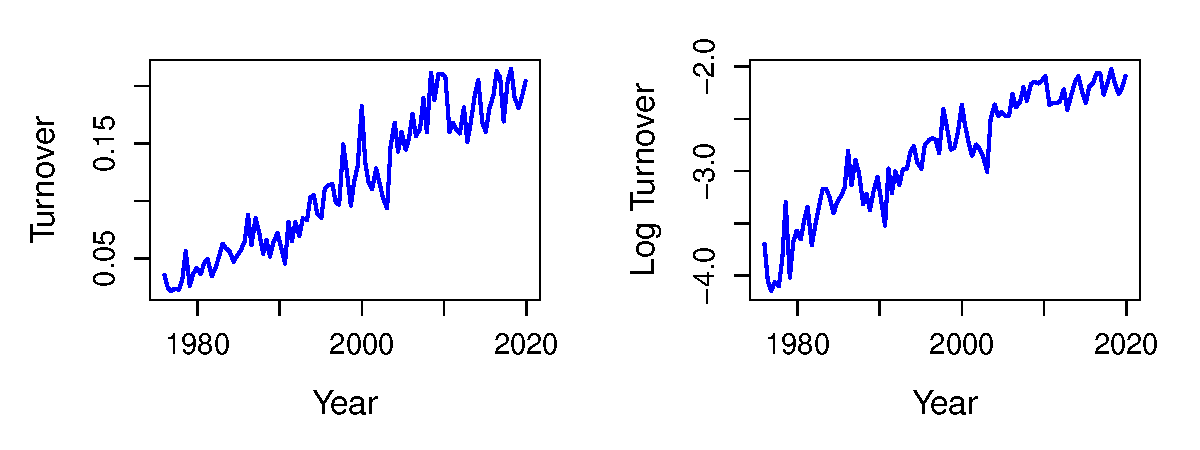
\includegraphics{turn_mean_trend.pdf}
\end{center}
\end{figure}

\clearpage 

\begin{figure}
\caption{Heatmap of Anomaly Correlations}
\label{fig:corr_plot_signals}
\subcaption*{A matrix heat map of pairwise correlations among the 39 anomaly signals. Blue circles represent positive correlations, while red circles are negative correlations. A bigger circle represents a higher magnitude of correlations. The lower half represents signals correlations, while the upper half represents signal rank correlations. Anomaly signals and their ranks are computed cross-section every month.}
\rule[0.25ex]{\linewidth}{1pt}
\begin{center}
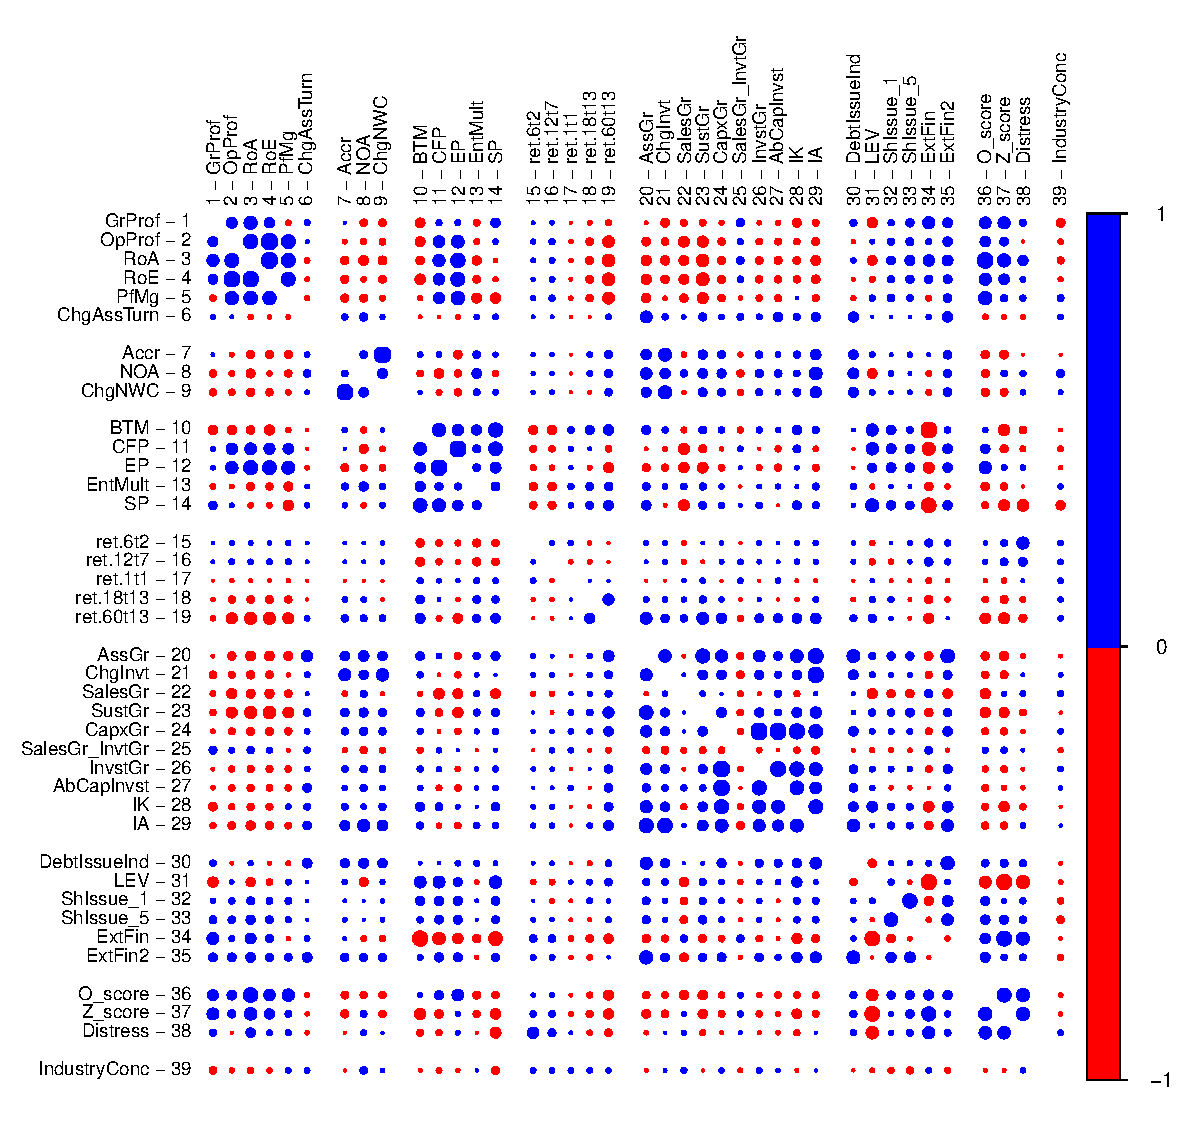
\includegraphics{corr_plot_signals.pdf}
\end{center}
\end{figure}

\clearpage 

\begin{figure}
\caption{Disagreement Trend}
\label{fig:std_dev_funda_trend}
\subcaption*{Monthly cross-sectional mean and standard error of the disagreement measure ($STD\_DEV$) over 1976--2019. The confidence interval is set to two standard errors.}
\rule[0.25ex]{\linewidth}{1pt}
\begin{center}
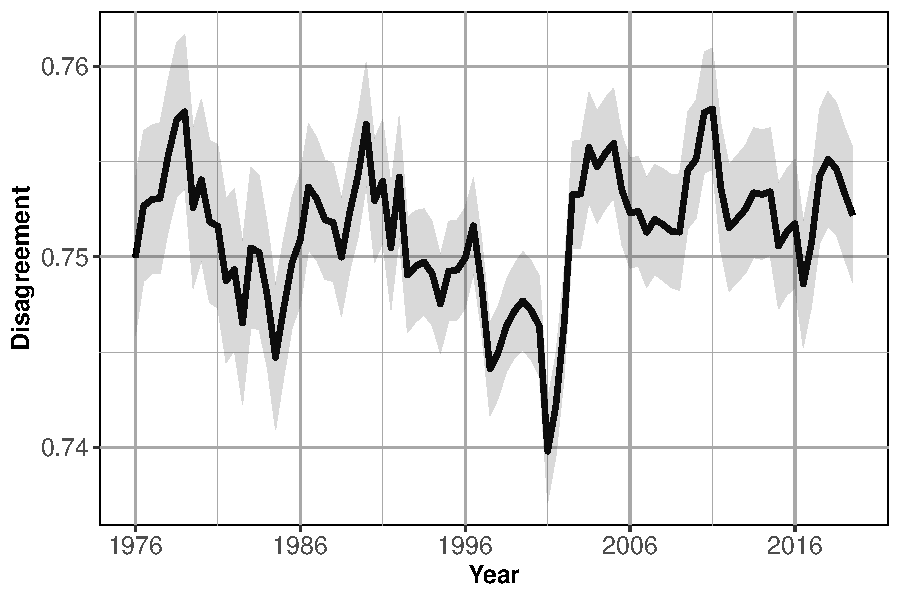
\includegraphics{std_dev_funda_trend.pdf}
\end{center}
\end{figure}

\clearpage 

\begin{figure}
\caption{Disagreement and Anomaly Groups}
\label{fig:disagreement_leave_one_out}
\subcaption*{Average monthly Disagreement, over the period 1976--2019, using all but one group of anomalies over time. The number in paranthesis represents the number of AFs skipped in constructing disagreement.}
\rule[0.25ex]{\linewidth}{1pt}
\begin{center}
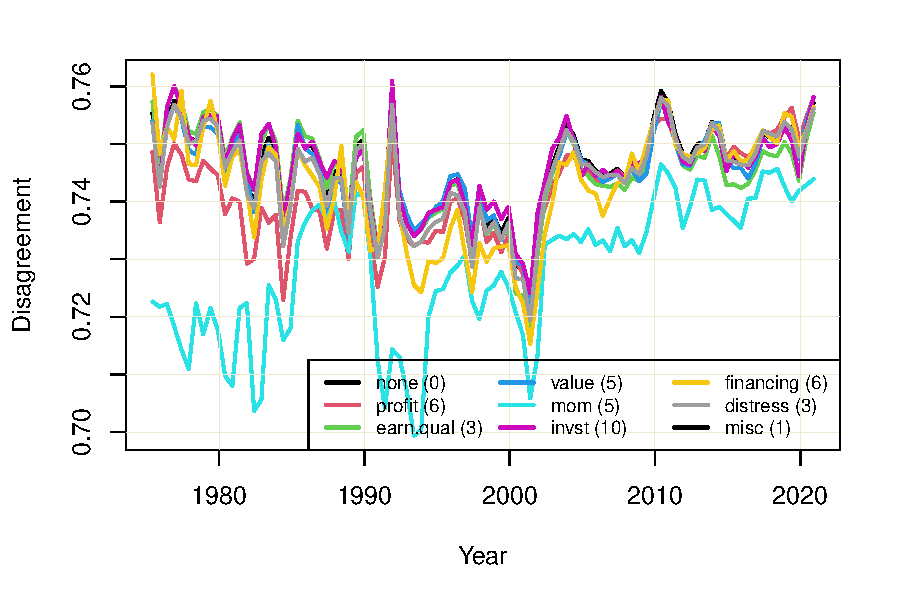
\includegraphics{disagreement_leave_one_out.pdf}
\end{center}
\end{figure}

\clearpage 

\newgeometry{margin=0.5in}
\begin{landscape}
\begin{figure}
\caption{Anomalies and Turnover}
\label{fig:anomaly_usage_evidence_2}
\subcaption*{Extreme decile (D1 and D10) and middle decile (D2 to D9) percentage returns, turnover ranks, disagreement-turnover ranks, and other-turnover ranks with respect to anomalies. Decile portfolios based on anomalies are constructed each month-end, and all variables are computed at the end of next month. Returns are monthly percentages, while turnover is in cross-sectional percentiles (100 $\times$ Ranks). Extreme decile turnover is $0.5 \times (TURN^{D1} + TURN^{D10})$ and intermediate decile turnover is $0.125 \times (TURN^{D2} + \dots + TURN^{D9})$. Disagreement- and excess-turnover is computed similarly.}
\rule[0.25ex]{\linewidth}{1pt}
\begin{center}
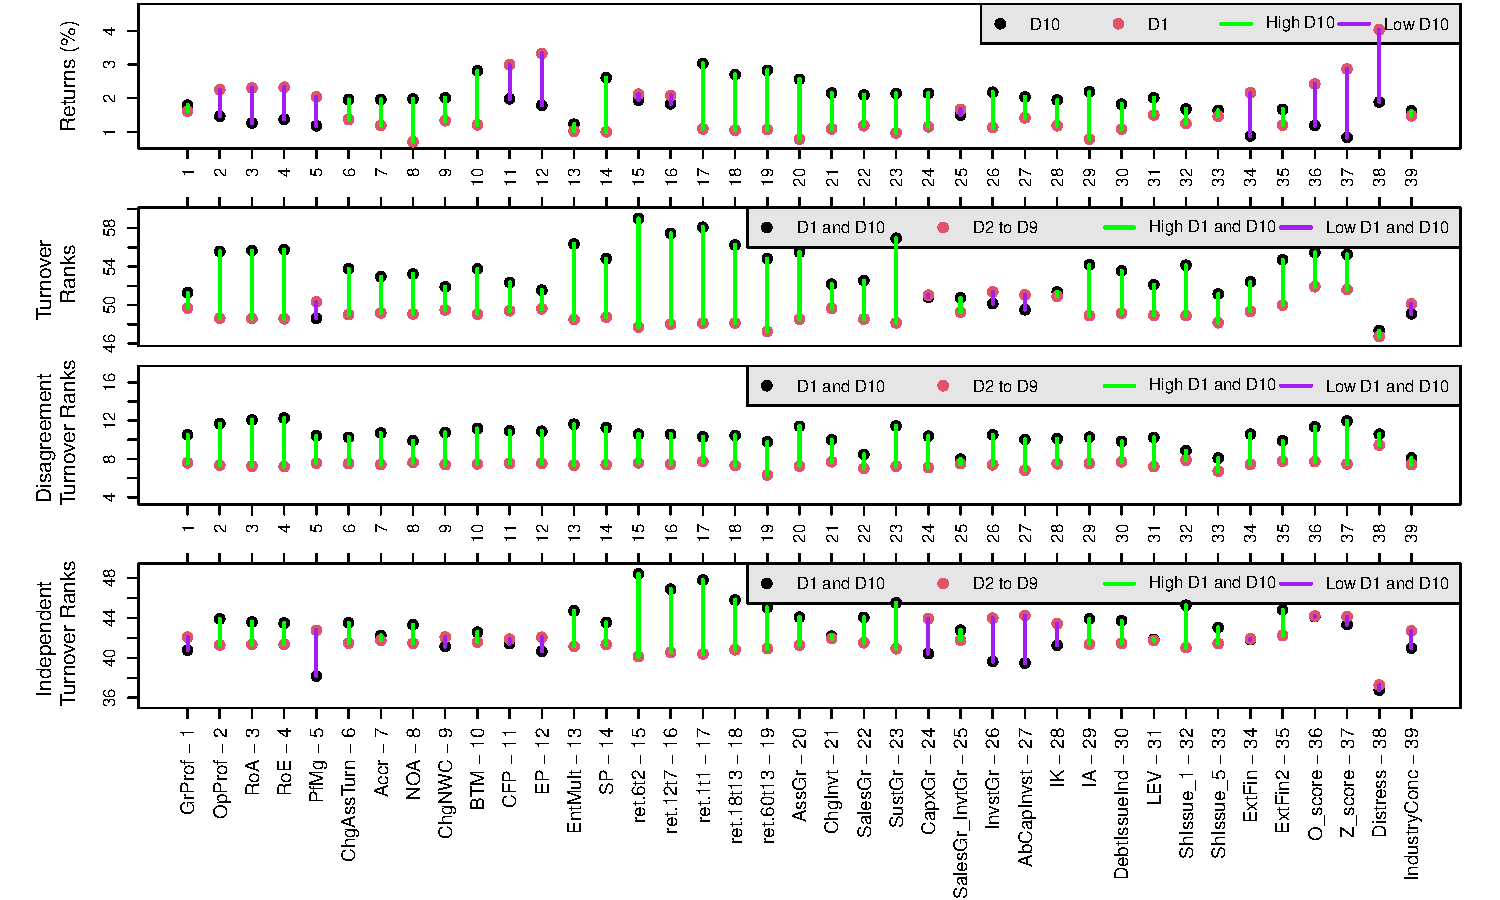
\includegraphics{anomaly_usage_evidence_2.pdf}
\end{center}
\end{figure}
\end{landscape}
\restoregeometry

\clearpage  \begingroup\fontsize{12}{14}\selectfont

\begin{spacing}{1.0}
\begin{longtable}[t]{>{\raggedleft\arraybackslash}p{1cm}>{\raggedright\arraybackslash}p{8cm}>{\raggedleft\arraybackslash}p{3cm}}
\caption[Anomaly Papers]{\label{tab:anomaly_paper_list}Anomaly Papers}\\
\multicolumn{3}{p{12cm}}{A brief list of anomaly papers and the number of anomalies used in the study.}\\
\toprule
\textbf{S.No.} & \textbf{Source} & \textbf{Number of Anomalies}\\
\midrule
\endfirsthead
\caption[]{Anomaly Papers \textit{(continued)}}\\
\toprule
\textbf{S.No.} & \textbf{Source} & \textbf{Number of Anomalies}\\
\midrule
\endhead

\endfoot
\bottomrule
\endlastfoot
1 & \cite*{stambaugh_etal_2012} & 11\\
2 & \cite*{roberts2018} & 34\\
3 & \cite*{green_etal_2017} & 94\\
4 & \cite*{mclean_pontiff2016} & 97\\
5 & \cite*{feng_etal_2020} & 150\\
6 & \cite*{chordia_etal_2020} & 185\\
7 & \cite*{harvey_etal2016} & 316\\
8 & \cite*{replicating_anomalies_2020} & 452\\*
\end{longtable}
\end{spacing}
\endgroup{}
 \clearpage 
\begingroup\fontsize{12}{14}\selectfont

\begin{spacing}{1.0}
\begin{longtable}[t]{>{\raggedright\arraybackslash}p{4.3cm}>{\centering\arraybackslash}p{2.6cm}>{\centering\arraybackslash}p{3.4cm}>{\centering\arraybackslash}p{3.4cm}}
\caption[Disagreement by Industry]{\label{tab:disagreement_by_industry}Disagreement by Industry}\\
\multicolumn{4}{p{\linewidth}}{Average disagreement ranks ($\times 100$) and its standard deviation across 48 FF industry classifications (\cite{fama_french_industry}). Only the top ten and bottom ten industries having the highest and lowest levels of average disagreement are shown. The second column shows the percentage of firm-months in the respective industry.}\\
\toprule
\textbf{Industry} & \textbf{\shortstack{\% Sample}} & \textbf{\shortstack{Avg. Disagreement \\ (Ranks)}} & \textbf{\shortstack{SD Disagreement \\ (Ranks)}}\\
\midrule
\endfirsthead
\caption[]{Disagreement by Industry \textit{(continued)}}\\
\toprule
\textbf{Industry} & \textbf{\shortstack{\% Sample}} & \textbf{\shortstack{Avg. Disagreement \\ (Ranks)}} & \textbf{\shortstack{SD Disagreement \\ (Ranks)}}\\
\midrule
\endhead

\endfoot
\bottomrule
\endlastfoot
\addlinespace[0.3em]
\multicolumn{4}{l}{\textbf{Top 10}}\\
\hspace{1em}Pharmaceuticals & 5.52 & 69.6 & 22.3\\
\hspace{1em}Precious-Metals & 0.28 & 59.9 & 23.9\\
\hspace{1em}Medical-Equipment & 2.88 & 58.1 & 25.8\\
\hspace{1em}Computers & 3.43 & 56.2 & 24.9\\
\hspace{1em}Real-Estate & 0.75 & 56.0 & 24.6\\
\hspace{1em}IT Services & 9.87 & 54.3 & 24.9\\
\hspace{1em}Construction & 1.27 & 53.4 & 24.3\\
\hspace{1em}Coal & 0.19 & 53.2 & 24.4\\
\hspace{1em}Trading & 2.30 & 52.9 & 23.5\\
\hspace{1em}Electronic Chips & 5.23 & 52.3 & 25.2\\
\addlinespace[0.3em]
\multicolumn{4}{l}{\textbf{Bottom 10}}\\
\hspace{1em}Automobiles & 1.48 & 40.9 & 24.7\\
\hspace{1em}Food-Products & 1.68 & 39.6 & 24.0\\
\hspace{1em}Publishing & 0.73 & 39.5 & 24.3\\
\hspace{1em}Beer-\&-Liquor & 0.32 & 39.0 & 23.3\\
\hspace{1em}Insurance & 3.28 & 37.5 & 22.3\\
\hspace{1em}Aircraft & 0.57 & 37.5 & 24.7\\
\hspace{1em}Chemicals & 1.83 & 37.2 & 25.9\\
\hspace{1em}Business-Supplies & 1.27 & 36.3 & 23.7\\
\hspace{1em}Shipping-Containers & 0.33 & 32.4 & 23.0\\
\hspace{1em}Utilities & 3.52 & 29.7 & 18.7\\*
\end{longtable}
\end{spacing}
\endgroup{}
 \clearpage

\begin{landscape}
\begingroup\fontsize{12}{14}\selectfont

\begin{spacing}{1.0}
\begin{longtable}[t]{>{\raggedright\arraybackslash}p{3.9cm}>{\raggedleft\arraybackslash}p{1.5cm}>{\raggedleft\arraybackslash}p{1.5cm}>{\raggedleft\arraybackslash}p{1.5cm}>{\raggedleft\arraybackslash}p{1.5cm}>{\raggedleft\arraybackslash}p{1.5cm}>{\raggedleft\arraybackslash}p{1.5cm}>{\raggedleft\arraybackslash}p{1.5cm}>{\raggedleft\arraybackslash}p{1.5cm}>{\raggedleft\arraybackslash}p{1.5cm}}
\caption[Correlations and Descriptive Statistics]{\label{tab:correlations_and_summary_stat_POOLED}Descriptive Statistics and Correlations}\\
\multicolumn{10}{p{\linewidth}}{\textbf{Panel A: Descriptive Statistics}}\\
\multicolumn{10}{p{\linewidth}}{Panel A presents pooled cross-section descriptive statistics of turnover and explanatory variables. Variable definitions are present in Appendix \ref{appendix-a2-variable-definitions}}\\
\toprule

  & \textbf{Mean} & \textbf{SD} & \textbf{Min} & \textbf{p25} & \textbf{Median} & \textbf{p75} & \textbf{Max} & \textbf{Skew} & \textbf{Kurt}\\
\midrule
\endfirsthead
\caption[]{Descriptive Statistics and Correlations \textit{(continued)}}\\
\toprule
  & \textbf{Mean} & \textbf{SD} & \textbf{Min} & \textbf{p25} & \textbf{Median} & \textbf{p75} & \textbf{Max} & \textbf{Skew} & \textbf{Kurt}\\
\midrule
\endhead

\endfoot
\bottomrule
\endlastfoot
$L\_TURN$ & $-2.73$ & $1.20$ & $-7.22$ & $-3.53$ & $-2.68$ & $-1.88$ & $1.56$ & $-0.17$ & $2.86$\\
$STD\_DEV$ & $0.75$ & $0.10$ & $0.43$ & $0.68$ & $0.75$ & $0.83$ & $0.99$ & $-0.20$ & $2.55$\\
$FDISP$ & $0.21$ & $0.63$ & $0.00$ & $0.02$ & $0.05$ & $0.14$ & $13.00$ & $7.44$ & $75.67$\\
$NASDAQ$ & $0.55$ & $0.50$ & $0.00$ & $0.00$ & $1.00$ & $1.00$ & $1.00$ & $-0.19$ & $1.04$\\
$RET^+$ & $0.05$ & $0.11$ & $0.00$ & $0.00$ & $0.00$ & $0.07$ & $2.56$ & $4.52$ & $41.00$\\
$RET^-$ & $-0.04$ & $0.08$ & $-0.70$ & $-0.06$ & $0.00$ & $0.00$ & $0.00$ & $-2.63$ & $11.46$\\
$LEV$ & $0.55$ & $1.35$ & $0.00$ & $0.01$ & $0.15$ & $0.52$ & $27.19$ & $6.60$ & $65.02$\\
$CAPM\_\beta$ & $1.27$ & $0.54$ & $0.08$ & $0.92$ & $1.26$ & $1.53$ & $2.88$ & $0.35$ & $2.72$\\
$BTM$ & $0.76$ & $0.92$ & $-2.56$ & $0.27$ & $0.55$ & $0.96$ & $18.95$ & $4.21$ & $36.50$\\
$L\_PRC$ & $2.54$ & $1.05$ & $0.00$ & $1.83$ & $2.67$ & $3.31$ & $6.34$ & $-0.27$ & $2.64$\\
$L\_FAGE$ & $4.40$ & $1.24$ & $0.00$ & $3.69$ & $4.63$ & $5.33$ & $6.54$ & $-0.90$ & $3.66$\\
$L\_ME$ & $19.06$ & $2.06$ & $13.67$ & $17.54$ & $18.90$ & $20.44$ & $26.27$ & $0.38$ & $2.82$\\
$ESURP$ & $0.04$ & $0.13$ & $0.00$ & $0.00$ & $0.01$ & $0.02$ & $4.28$ & $10.81$ & $176.54$\\
$EVOL$ & $0.04$ & $0.14$ & $0.00$ & $0.00$ & $0.01$ & $0.03$ & $4.27$ & $10.88$ & $178.90$\\
$NUMEST$ & $6.83$ & $7.02$ & $1.00$ & $2.00$ & $4.00$ & $9.00$ & $56.00$ & $1.74$ & $6.15$\\*
\end{longtable}
\end{spacing}
\endgroup{}
\clearpage
\begingroup\fontsize{12}{14}\selectfont

\begin{spacing}{1.0}
\begin{longtable}{>{\raggedright\arraybackslash}p{2.8cm}>{\raggedright\arraybackslash}p{0.8cm}>{\raggedright\arraybackslash}p{0.8cm}>{\raggedright\arraybackslash}p{0.8cm}>{\raggedright\arraybackslash}p{0.8cm}>{\raggedright\arraybackslash}p{0.8cm}>{\raggedright\arraybackslash}p{0.8cm}>{\raggedright\arraybackslash}p{0.8cm}>{\raggedright\arraybackslash}p{0.8cm}>{\raggedright\arraybackslash}p{0.8cm}>{\raggedright\arraybackslash}p{0.8cm}>{\raggedright\arraybackslash}p{0.8cm}>{\raggedright\arraybackslash}p{0.8cm}>{\raggedright\arraybackslash}p{0.8cm}>{\raggedright\arraybackslash}p{0.8cm}>{\raggedright\arraybackslash}p{0.8cm}}
\multicolumn{16}{p{\linewidth}}{\textbf{Panel B: Correlations}}\\
\multicolumn{16}{p{\linewidth}}{Panel B reports pooled cross-section correlation coefficients. The lower triangle represents variable correlation, while the upper triangle consists of rank correlations. Variable definitions are present in Appendix \ref{appendix-a2-variable-definitions}}\\
\toprule

  & $\phantom{--}(1)$ & $\phantom{--}(2)$ & $\phantom{--}(3)$ & $\phantom{--}(4)$ & $\phantom{--}(5)$ & $\phantom{--}(6)$ & $\phantom{--}(7)$ & $\phantom{--}(8)$ & $\phantom{--}(9)$ & $\phantom{-}(10)$ & $\phantom{-}(11)$ & $\phantom{-}(12)$ & $\phantom{-}(13)$ & $\phantom{-}(14)$ & $\phantom{-}(15)$\\
\midrule
\endfirsthead
\caption[]{Descriptive Statistics and Correlations \textit{(continued)}}\\
\toprule
  & $\phantom{--}(1)$ & $\phantom{--}(2)$ & $\phantom{--}(3)$ & $\phantom{--}(4)$ & $\phantom{--}(5)$ & $\phantom{--}(6)$ & $\phantom{--}(7)$ & $\phantom{--}(8)$ & $\phantom{--}(9)$ & $\phantom{-}(10)$ & $\phantom{-}(11)$ & $\phantom{-}(12)$ & $\phantom{-}(13)$ & $\phantom{-}(14)$ & $\phantom{-}(15)$\\
\midrule
\endhead

\endfoot
\bottomrule
\endlastfoot
$(1)\phantom{--}L\_TURN$ &  & $\phantom{-}0.16$ & $\phantom{-}0.05$ & $\phantom{-}0.03$ & $\phantom{-}0.16$ & $-0.05$ & $-0.08$ & $\phantom{-}0.01$ & $-0.22$ & $\phantom{-}0.17$ & $-0.04$ & $\phantom{-}0.30$ & $\phantom{-}0.02$ & $-0.03$ & $\phantom{-}0.29$\\
$(2)\phantom{--}STD\_DEV$ & $\phantom{-}0.14$ &  & $\phantom{-}0.14$ & $\phantom{-}0.20$ & $\phantom{-}0.12$ & $-0.18$ & $\phantom{-}0.10$ & $\phantom{-}0.02$ & $-0.01$ & $-0.39$ & $-0.27$ & $-0.28$ & $\phantom{-}0.19$ & $\phantom{-}0.21$ & $-0.15$\\
$(3)\phantom{--}FDISP$ & $\phantom{-}0.00$ & $\phantom{-}0.27$ &  & $\phantom{-}0.04$ & $\phantom{-}0.04$ & $-0.06$ & $\phantom{-}0.08$ & $-0.02$ & $\phantom{-}0.10$ & $-0.23$ & $-0.10$ & $-0.34$ & $\phantom{-}0.10$ & $\phantom{-}0.10$ & $-0.11$\\
$(4)\phantom{--}NASDAQ$ & $\phantom{-}0.12$ & $\phantom{-}0.20$ & $\phantom{-}0.10$ &  & $\phantom{-}0.00$ & $-0.05$ & $-0.27$ & $\phantom{-}0.10$ & $-0.08$ & $-0.24$ & $-0.52$ & $-0.34$ & $\phantom{-}0.05$ & $\phantom{-}0.03$ & $-0.32$\\
$(5)\phantom{--}RET^+$ & $\phantom{-}0.18$ & $\phantom{-}0.07$ & $\phantom{-}0.03$ & $\phantom{-}0.05$ &  & $\phantom{-}0.53$ & $-0.05$ & $\phantom{-}0.00$ & $-0.11$ & $\phantom{-}0.06$ & $-0.01$ & $\phantom{-}0.06$ & $\phantom{-}0.05$ & $\phantom{-}0.03$ & $-0.01$\\
$(6)\phantom{--}RET^-$ & $-0.10$ & $-0.18$ & $-0.12$ & $-0.08$ & $\phantom{-}0.27$ &  & $\phantom{-}0.02$ & $-0.01$ & $-0.03$ & $\phantom{-}0.18$ & $\phantom{-}0.08$ & $\phantom{-}0.10$ & $-0.08$ & $-0.09$ & $\phantom{-}0.06$\\
$(7)\phantom{--}LEV$ & $-0.04$ & $-0.16$ & $\phantom{-}0.05$ & $-0.13$ & $-0.01$ & $-0.07$ &  & $-0.02$ & $\phantom{-}0.38$ & $-0.03$ & $\phantom{-}0.19$ & $\phantom{-}0.04$ & $\phantom{-}0.15$ & $\phantom{-}0.24$ & $\phantom{-}0.05$\\
$(8)\phantom{--}CAPM\_\beta$ & $\phantom{-}0.19$ & $-0.01$ & $\phantom{-}0.00$ & $\phantom{-}0.09$ & $-0.06$ & $\phantom{-}0.03$ & $-0.04$ &  & $\phantom{-}0.00$ & $\phantom{-}0.07$ & $-0.08$ & $\phantom{-}0.00$ & $-0.01$ & $-0.01$ & $-0.01$\\
$(9)\phantom{--}BTM$ & $-0.13$ & $-0.21$ & $\phantom{-}0.16$ & $-0.12$ & $-0.05$ & $-0.08$ & $\phantom{-}0.45$ & $-0.09$ &  & $-0.21$ & $\phantom{-}0.15$ & $-0.25$ & $\phantom{-}0.23$ & $\phantom{-}0.33$ & $-0.12$\\
$(10)\phantom{-}L\_PRC$ & $\phantom{-}0.18$ & $-0.36$ & $-0.39$ & $-0.25$ & $-0.04$ & $\phantom{-}0.23$ & $-0.16$ & $\phantom{-}0.10$ & $-0.24$ &  & $\phantom{-}0.30$ & $\phantom{-}0.73$ & $-0.42$ & $-0.51$ & $\phantom{-}0.51$\\
$(11)\phantom{-}L\_FAGE$ & $\phantom{-}0.00$ & $-0.28$ & $-0.03$ & $-0.36$ & $-0.05$ & $\phantom{-}0.09$ & $\phantom{-}0.05$ & $\phantom{-}0.15$ & $\phantom{-}0.10$ & $\phantom{-}0.23$ &  & $\phantom{-}0.32$ & $-0.03$ & $-0.04$ & $\phantom{-}0.28$\\
$(12)\phantom{-}L\_ME$ & $\phantom{-}0.37$ & $-0.31$ & $-0.17$ & $-0.27$ & $-0.02$ & $\phantom{-}0.10$ & $-0.12$ & $\phantom{-}0.20$ & $-0.26$ & $\phantom{-}0.74$ & $\phantom{-}0.33$ &  & $-0.16$ & $-0.17$ & $\phantom{-}0.73$\\
$(13)\phantom{-}ESURP$ & $\phantom{-}0.04$ & $\phantom{-}0.29$ & $\phantom{-}0.39$ & $\phantom{-}0.03$ & $\phantom{-}0.08$ & $-0.07$ & $\phantom{-}0.24$ & $-0.02$ & $\phantom{-}0.21$ & $-0.26$ & $-0.08$ & $-0.37$ &  & $\phantom{-}0.68$ & $-0.21$\\
$(14)\phantom{-}EVOL$ & $\phantom{-}0.03$ & $\phantom{-}0.31$ & $\phantom{-}0.45$ & $\phantom{-}0.03$ & $\phantom{-}0.09$ & $-0.06$ & $\phantom{-}0.27$ & $-0.02$ & $\phantom{-}0.20$ & $-0.28$ & $-0.05$ & $-0.45$ & $\phantom{-}0.67$ &  & $-0.25$\\
$(15)\phantom{-}NUMEST$ & $\phantom{-}0.27$ & $-0.16$ & $-0.18$ & $-0.31$ & $-0.06$ & $\phantom{-}0.07$ & $-0.04$ & $\phantom{-}0.05$ & $-0.08$ & $\phantom{-}0.49$ & $\phantom{-}0.34$ & $\phantom{-}0.68$ & $-0.09$ & $-0.10$ & \\*
\end{longtable}
\end{spacing}
\endgroup{}
\end{landscape}
 \clearpage

\begin{landscape}
\begingroup\fontsize{12}{14}\selectfont

\begin{spacing}{1.0}
\begin{xltabular}{\linewidth}{X * {9}{S[table-format=5.3]}}
\caption[Regression: Different Specifications]{\label{tab:reg_compact_main}Cross-sectional regression: different specifications}\\
\multicolumn{10}{p{\linewidth}}{Log turnover regressed on lagged disagreement and controls. $L\_TURN_{i,t} = \beta \cdot STD\_DEV_{i,t-1} + \alpha \cdot CONTROLS_{i,t-1} + \gamma \cdot DUMMIES_{i,t-1} + \epsilon_{i,t}$. Specification (5) uses 80/20 stock splits to compute disagreement, while others use 70/30 split. In specification (6), I compute disagreement by excluding all momentum signals viz. $ret.6t2$, $ret.12t7$, $ret.1t1$, $ret.18t13$, and $ret.60t13$. In specification (7), all dependent variables except $NASDAQ$ dummy and $NUMEST$ are converted to their respective cross-sectional ranks. Specification (8) and (9) has log turnover computed on the following day and week (5 days), respectively. Specification (3) has 256,507 firm-months of observations while all other specifications have 872,061 firm-months. All independent variables are one-month lagged variables. Definitions of all the variables appear in Appendix \ref{appendix-a2-variable-definitions}. All regression specifications have industry and year fixed effects. \textit{t}-statistics are present in paranthesis based on standard errors double clustered by firm and year-month. Statistical significance of 10\%, 5\% and 1\% are indicated by *, ** and *** respectively.}\\
\toprule

\multicolumn{1}{c}{\bgroup\fontsize{12}{14}\selectfont  \egroup{}} & \multicolumn{6}{c}{\bgroup\fontsize{12}{14}\selectfont \makecell{Monthly $L\_TURN$}\egroup{}} & \multicolumn{1}{c}{\bgroup\fontsize{12}{14}\selectfont \makecell{$TURN$ \\ Rank}\egroup{}} & \multicolumn{1}{c}{\bgroup\fontsize{12}{14}\selectfont \makecell{Next-day \\ $L\_TURN$}\egroup{}} & \multicolumn{1}{c}{\bgroup\fontsize{12}{14}\selectfont \makecell{Next-week \\ $L\_TURN$}\egroup{}} \\
\cmidrule(l{3pt}r{3pt}){2-7} \cmidrule(l{3pt}r{3pt}){8-8} \cmidrule(l{3pt}r{3pt}){9-9} \cmidrule(l{3pt}r{3pt}){10-10}
 & {(1)} & {(2)} & {(3)} & {(4)} & {(5)} & {(6)} & {(7)} & {(8)} & {(9)}\\
\midrule
\endfirsthead
\caption[]{Cross-sectional regression: different specifications \textit{(continued)}}\\
\toprule
 & {(1)} & {(2)} & {(3)} & {(4)} & {(5)} & {(6)} & {(7)} & {(8)} & {(9)}\\
\midrule
\endhead

\endfoot
\bottomrule
\endlastfoot
$STD\_DEV$ &  & 1.545*** & 1.272*** & 1.557*** & 1.460*** & 1.092*** & 0.139*** & 1.499*** & 1.536***\\
 &  & (24.067) & (15.226) & (24.419) & (28.262) & (18.766) & (19.566) & (21.862) & (23.198)\\
\addlinespace
$FDISP$ & 0.030*** & 0.011* &  & 0.013** & 0.009 & 0.016** & 0.034*** & 0.007 & 0.008\\
 & (4.498) & (1.743) &  & (1.997) & (1.384) & (2.493) & (5.508) & (0.999) & (1.172)\\
\addlinespace
$PRC\_DISP$ &  &  & 1.009*** &  &  &  &  &  & \\
 &  &  & (14.318) &  &  &  &  &  & \\
\addlinespace
$L\_ME$ &  &  &  & 0.107*** &  &  &  &  & \\
 &  &  &  & (9.970) &  &  &  &  & \\
\addlinespace
$NASDAQ$ & 0.141*** & 0.122*** & 0.009 & 0.165*** & 0.118*** & 0.127*** & 0.040*** & 0.069*** & 0.098***\\
 & (6.175) & (5.430) & (0.322) & (7.538) & (5.309) & (5.641) & (6.482) & (3.050) & (4.301)\\
\addlinespace
$RET^+$ & 1.701*** & 1.522*** & 1.094*** & 1.521*** & 1.457*** & 1.625*** & 0.126*** & 2.385*** & 2.028***\\
 & (25.922) & (25.529) & (17.233) & (25.201) & (25.269) & (25.874) & (46.224) & (26.646) & (28.155)\\
\addlinespace
$RET^-$ & -2.438*** & -2.210*** & -2.014*** & -2.214*** & -2.116*** & -2.342*** & -0.154*** & -3.238*** & -2.779***\\
 & (-29.884) & (-29.507) & (-22.778) & (-29.303) & (-29.057) & (-29.891) & (-47.884) & (-36.001) & (-36.772)\\
\addlinespace
$LEV$ & 0.076*** & 0.062*** & 0.025** & 0.059*** & 0.053*** & 0.065*** & 0.087*** & 0.063*** & 0.062***\\
 & (9.601) & (8.189) & (2.272) & (7.825) & (7.180) & (8.540) & (11.398) & (7.730) & (7.844)\\
\addlinespace
$CAPM\_\beta$ & 0.081** & 0.085*** & 0.119*** & 0.080*** & 0.087*** & 0.085*** & 0.008 & 0.116** & 0.092***\\
 & (2.524) & (2.813) & (3.269) & (2.619) & (2.940) & (2.733) & (1.263) & (2.362) & (2.816)\\
\addlinespace
$BTM$ & 0.002 & 0.024* & -0.019 & 0.048*** & 0.028** & 0.018 & -0.061*** & 0.006 & 0.018\\
 & (0.128) & (1.871) & (-1.089) & (3.764) & (2.186) & (1.351) & (-6.726) & (0.410) & (1.314)\\
\addlinespace
$L\_PRC$ & 0.192*** & 0.229*** & 0.176*** & 0.148*** & 0.242*** & 0.218*** & 0.221*** & 0.304*** & 0.264***\\
 & (16.253) & (19.148) & (11.145) & (10.638) & (20.212) & (18.217) & (18.994) & (23.458) & (21.468)\\
\addlinespace
$L\_FAGE$ & -0.160*** & -0.134*** & -0.108*** & -0.156*** & -0.124*** & -0.143*** & -0.098*** & -0.099*** & -0.128***\\
 & (-12.253) & (-10.547) & (-6.119) & (-11.895) & (-9.809) & (-11.135) & (-9.845) & (-7.302) & (-9.751)\\
\addlinespace
$ESURP$ & 0.277*** & 0.232*** & 0.174*** & 0.220*** & 0.218*** & 0.248*** & 0.069*** & 0.222*** & 0.255***\\
 & (7.631) & (7.005) & (3.716) & (6.420) & (6.807) & (7.273) & (22.049) & (5.607) & (6.979)\\
\addlinespace
$EVOL$ & 0.148*** & 0.021 & 0.197** & 0.021 & -0.029 & 0.055 & 0.048*** & -0.053 & -0.038\\
 & (3.059) & (0.443) & (2.391) & (0.441) & (-0.603) & (1.161) & (6.307) & (-1.002) & (-0.756)\\
\addlinespace
$NUMEST$ & 0.035*** & 0.033*** & 0.024*** & 0.020*** & 0.034*** & 0.033*** & 0.010*** & 0.038*** & 0.035***\\
 & (23.284) & (22.717) & (13.175) & (12.029) & (23.029) & (22.716) & (24.610) & (24.894) & (23.541)\\
\midrule
$\textrm{Adj.} \: R^2$ & 0.392 & 0.407 & 0.360 & 0.413 & 0.413 & 0.401 & 0.289 & 0.374 & 0.391\\*
\end{xltabular}
\end{spacing}
\endgroup{}
\end{landscape}
 \clearpage

\begin{spacing}{1.0}
\begin{table}



\caption[Regression: Different Measures of Turnover]{\label{tab:reg_compact_diff_turn}Cross-sectional regression: different measures of turnover}
\centering
\fontsize{11}{13}\selectfont
\begin{tabularx}{\linewidth}{X * {5}{S[table-format=4.3]}}
\multicolumn{6}{p{\linewidth}}{Different measures of turnover regressed on lagged disagreement and controls. $TURNOVER_{i,t} = \beta \cdot STD\_DEV_{i,t-1} + \alpha \cdot CONTROLS_{i,t-1} + \gamma \cdot DUMMIES_{i,t-1} + \epsilon_{i,t}$. $\Delta L\_TURN_t$ is $L\_TURN_{i,t} - L\_TURN_{i,t-1}$, GRT adj. $L\_TURN$ is adjusted log turnover proposed by \citetalias{chordia_etal2006} and, VW $L\_TURN$ (EW $L\_TURN$) is the residual from regressing $L\_TURN$ on value-weighted (equal-weighted) market turnover. All specifications have 947,909 firm-month observations. All independent variables are one-month lagged variables. Definitions of all the variables appear in Appendix \ref{appendix-a2-variable-definitions}. All regression specifications have industry and year fixed effects. \textit{t}-statistics are present in paranthesis based on standard errors double clustered by firm and year-month. Statistical significance of 10\%, 5\% and 1\% are indicated by *, ** and *** respectively.}\\
\toprule

\multicolumn{1}{c}{\bgroup\fontsize{11}{13}\selectfont  \egroup{}} & \multicolumn{1}{c}{\bgroup\fontsize{11}{13}\selectfont $L\_TURN$\egroup{}} & \multicolumn{1}{c}{\bgroup\fontsize{11}{13}\selectfont $\Delta L\_TURN$\egroup{}} & \multicolumn{1}{c}{\bgroup\fontsize{11}{13}\selectfont \makecell{GRT adj. \\ $L\_TURN$}\egroup{}} & \multicolumn{1}{c}{\bgroup\fontsize{11}{13}\selectfont \makecell{VW \\ $L\_TURN$}\egroup{}} & \multicolumn{1}{c}{\bgroup\fontsize{11}{13}\selectfont \makecell{EW \\ $L\_TURN$}\egroup{}} \\
\cmidrule(l{3pt}r{3pt}){2-2} \cmidrule(l{3pt}r{3pt}){3-3} \cmidrule(l{3pt}r{3pt}){4-4} \cmidrule(l{3pt}r{3pt}){5-5} \cmidrule(l{3pt}r{3pt}){6-6}
 & {(1)} & {(2)} & {(3)} & {(4)} & {(5)}\\
\midrule
$STD\_DEV$ & 1.575*** & 0.022** & 0.941*** & 0.504*** & 0.512***\\
 & (25.522) & (2.533) & (16.520) & (17.909) & (18.282)\\
\addlinespace
$FDISP$ & 0.010 & -0.003*** & 0.013** & -0.006* & -0.008**\\
 & (1.638) & (-3.106) & (2.212) & (-1.797) & (-2.311)\\
\addlinespace
$NASDAQ$ & 0.128*** & 0.001 & 0.110*** & 0.069*** & 0.057***\\
 & (5.828) & (0.721) & (5.880) & (8.174) & (6.326)\\
\addlinespace
$RET^+$ & 1.497*** & -0.744*** & 0.753*** & 0.992*** & 0.969***\\
 & (24.849) & (-18.660) & (18.823) & (20.202) & (21.558)\\
\addlinespace
$RET^-$ & -2.144*** & 0.710*** & -0.899*** & -1.381*** & -1.531***\\
 & (-28.905) & (11.784) & (-14.538) & (-25.452) & (-33.715)\\
\addlinespace
$LEV$ & 0.062*** & 0.002*** & 0.045*** & 0.014*** & 0.015***\\
 & (9.116) & (4.064) & (7.405) & (5.091) & (5.157)\\
\addlinespace
$CAPM\_\beta$ & 0.086*** & 0.038 & 0.011 & 0.056** & 0.016\\
 & (2.902) & (1.002) & (0.374) & (2.320) & (0.774)\\
\addlinespace
$BTM$ & 0.024** & 0.002 & 0.050*** & -0.010** & -0.010**\\
 & (2.048) & (1.354) & (4.664) & (-2.005) & (-2.159)\\
\addlinespace
$L\_PRC$ & 0.229*** & -0.015*** & 0.095*** & 0.124*** & 0.135***\\
 & (19.331) & (-5.469) & (9.779) & (19.714) & (19.561)\\
\addlinespace
$L\_FAGE$ & -0.130*** & -0.005*** & -0.421*** & 0.002 & 0.007\\
 & (-10.652) & (-3.534) & (-30.552) & (0.469) & (1.644)\\
\addlinespace
$ESURP$ & 0.245*** & 0.025** & 0.077*** & 0.116*** & 0.144***\\
 & (7.764) & (2.181) & (2.889) & (5.967) & (7.860)\\
\addlinespace
$EVOL$ & 0.000 & 0.014 & 0.177*** & -0.083*** & -0.101***\\
 & (0.007) & (1.049) & (4.661) & (-2.819) & (-3.194)\\
\addlinespace
$NUMEST$ & 0.033*** & 0.000 & 0.031*** & -0.001*** & 0.000\\
 & (23.747) & (0.280) & (23.327) & (-2.631) & (0.873)\\
\midrule
$\textrm{Adj.} \: R^2$ & 0.404 & 0.018 & 0.243 & 0.083 & 0.088\\
\bottomrule
\end{tabularx}

\end{table}
\end{spacing}
 \clearpage

\begin{landscape}
\begingroup\fontsize{12}{14}\selectfont

\begin{spacing}{1.0}
\begin{longtable}[t]{>{\raggedright\arraybackslash}p{4.4cm}>{\raggedleft\arraybackslash}p{1.5cm}>{\raggedleft\arraybackslash}p{1.5cm}>{\raggedleft\arraybackslash}p{1.5cm}>{\raggedleft\arraybackslash}p{1.5cm}>{\raggedleft\arraybackslash}p{1.5cm}>{\raggedleft\arraybackslash}p{1.5cm}>{\raggedleft\arraybackslash}p{1.5cm}>{\raggedleft\arraybackslash}p{1.5cm}>{\raggedleft\arraybackslash}p{1.5cm}}
\caption[Descriptive Statistics and Correlations]{\label{tab:inf_env_corr_and_dstats_POOLED}Descriptive Statistics and Correlations}\\
\multicolumn{10}{p{\linewidth}}{\textbf{Panel A: Descriptive Statistics}}\\
\multicolumn{10}{p{\linewidth}}{Pooled cross-section descriptive statistics of information quality variables. $DOC\_SIZE$ is the size of raw 10-K filing in megabytes, $LENGTH$ (in 1000s) is the number of words in a 10-K document and, $CMP\_WORDS$ is the number of unique occurrences of 374 complex words identified in \cite{lm_2020_firm_complexity}. Variable definitions are present in Appendix \ref{appendix-a2-variable-definitions}.}\\
\toprule

  & \textbf{Mean} & \textbf{SD} & \textbf{Min} & \textbf{p25} & \textbf{Median} & \textbf{p75} & \textbf{Max} & \textbf{Skew} & \textbf{Kurt}\\
\midrule
\endfirsthead
\caption[]{Descriptive Statistics and Correlations \textit{(continued)}}\\
\toprule
  & \textbf{Mean} & \textbf{SD} & \textbf{Min} & \textbf{p25} & \textbf{Median} & \textbf{p75} & \textbf{Max} & \textbf{Skew} & \textbf{Kurt}\\
\midrule
\endhead

\endfoot
\bottomrule
\endlastfoot
$DOC\_SIZE$ & $5.85$ & $10.81$ & $0.00$ & $0.38$ & $1.32$ & $6.83$ & $434.66$ & $6.50$ & $139.54$\\
$LENGTH$ & $47.33$ & $36.46$ & $0.01$ & $25.89$ & $39.16$ & $57.46$ & $1530.66$ & $4.87$ & $78.57$\\
$CMP\_WORDS$ & $81.45$ & $21.07$ & $16.00$ & $66.00$ & $80.00$ & $95.00$ & $177.00$ & $0.32$ & $3.15$\\
$L\_ME$ & $19.06$ & $2.06$ & $13.67$ & $17.54$ & $18.90$ & $20.44$ & $26.27$ & $0.38$ & $2.82$\\
$L\_FAGE$ & $4.40$ & $1.24$ & $0.00$ & $3.69$ & $4.63$ & $5.33$ & $6.54$ & $-0.90$ & $3.66$\\
$NUMEST$ & $6.83$ & $7.02$ & $1.00$ & $2.00$ & $4.00$ & $9.00$ & $56.00$ & $1.74$ & $6.15$\\*
\end{longtable}
\end{spacing}
\endgroup{}\begingroup\fontsize{12}{14}\selectfont

\begin{spacing}{1.0}
\begin{longtable}{>{\raggedright\arraybackslash}p{8.7cm}>{\raggedright\arraybackslash}p{1.7cm}>{\raggedright\arraybackslash}p{1.7cm}>{\raggedright\arraybackslash}p{1.7cm}>{\raggedright\arraybackslash}p{1.7cm}>{\raggedright\arraybackslash}p{1.7cm}>{\raggedright\arraybackslash}p{1.7cm}}
\multicolumn{7}{p{\linewidth}}{\textbf{Panel B: Correlations}}\\
\multicolumn{7}{p{\linewidth}}{Pooled cross-section correlation coefficients. The lower triangle represents variable correlation, while the upper triangle consists of rank correlations. Variable definitions are present in Appendix \ref{appendix-a2-variable-definitions}}\\
\toprule

  & $\phantom{--}(1)$ & $\phantom{--}(2)$ & $\phantom{--}(3)$ & $\phantom{--}(4)$ & $\phantom{--}(5)$ & $\phantom{--}(6)$\\
\midrule
\endfirsthead
\caption[]{Descriptive Statistics and Correlations \textit{(continued)}}\\
\toprule
  & $\phantom{--}(1)$ & $\phantom{--}(2)$ & $\phantom{--}(3)$ & $\phantom{--}(4)$ & $\phantom{--}(5)$ & $\phantom{--}(6)$\\
\midrule
\endhead

\endfoot
\bottomrule
\endlastfoot
$(1)\phantom{--}DOC\_SIZE$ &  & $\phantom{-}0.65$ & $\phantom{-}0.42$ & $\phantom{-}0.37$ & $\phantom{-}0.20$ & $\phantom{-}0.21$\\
$(2)\phantom{--}LENGTH$ & $\phantom{-}0.33$ &  & $\phantom{-}0.81$ & $\phantom{-}0.33$ & $\phantom{-}0.04$ & $\phantom{-}0.22$\\
$(3)\phantom{--}CMP\_WORDS$ & $\phantom{-}0.31$ & $\phantom{-}0.73$ &  & $\phantom{-}0.34$ & $-0.05$ & $\phantom{-}0.28$\\
$(4)\phantom{--}L\_ME$ & $\phantom{-}0.32$ & $\phantom{-}0.31$ & $\phantom{-}0.38$ &  & $\phantom{-}0.33$ & $\phantom{-}0.73$\\
$(5)\phantom{--}L\_FAGE$ & $\phantom{-}0.12$ & $-0.01$ & $-0.03$ & $\phantom{-}0.32$ &  & $\phantom{-}0.28$\\
$(6)\phantom{--}NUMEST$ & $\phantom{-}0.27$ & $\phantom{-}0.25$ & $\phantom{-}0.26$ & $\phantom{-}0.68$ & $\phantom{-}0.34$ & \\*
\end{longtable}
\end{spacing}
\endgroup{}
\end{landscape}
 \clearpage 
\begingroup\fontsize{12}{14}\selectfont

\begin{spacing}{1.0}
\begin{longtable}[t]{>{\raggedright\arraybackslash}p{6.5cm}>{\raggedright\arraybackslash}p{2.2cm}>{\raggedright\arraybackslash}p{2.2cm}>{\raggedright\arraybackslash}p{2.2cm}}
\caption[Information Environment: Summary of Regression Splits]{\label{tab:reg_all_info_env_together}Information Environment: Summary of Regression Splits}\\
\multicolumn{4}{p{\linewidth}}{The table summarizes turnover regressions across portfolios made using several variables related to the firm's information environment. Two sets of regressions corresponding to specifications 1 and 2 of Table \ref{tab:reg_compact_main} are estimated for each portfolio. Forecast dispersion is included in both regressions. Other explanatory variables (Table \ref{tab:reg_compact_main}), standard errors, and $R^2$ statistics are skipped for brevity. Definitions of all the variables appear in Appendix \ref{appendix-a2-variable-definitions}. All regression specifications have industry and year fixed effects. Standard errors are double clustered by firm and year-month. Statistical significance of 10\%, 5\% and 1\% are indicated by *, ** and *** respectively.}\\
\toprule
\multicolumn{1}{c}{\textbf{\makecell{Portfolio Criterion}}} & \multicolumn{1}{c}{\textbf{w/o STD\_DEV}} & \multicolumn{2}{c}{\textbf{with STD\_DEV}} \\
\cmidrule(l{3pt}r{3pt}){1-1} \cmidrule(l{3pt}r{3pt}){2-2} \cmidrule(l{3pt}r{3pt}){3-4}
\multicolumn{1}{c}{ } & \multicolumn{1}{c}{$FDISP_{t-1}$} & \multicolumn{1}{c}{$FDISP_{t-1}$} & \multicolumn{1}{c}{$STD\_DEV_{t-1}$} \\
\cmidrule(l{3pt}r{3pt}){2-2} \cmidrule(l{3pt}r{3pt}){3-3} \cmidrule(l{3pt}r{3pt}){4-4}
\endfirsthead
\caption[]{Information Environment: Summary of Regression Splits \textit{(continued)}}\\
\toprule
\endhead

\endfoot
\bottomrule
\endlastfoot
\addlinespace[0.3em]
\multicolumn{4}{l}{\textbf{10-K Document Size}}\\
\hspace{1em}$DOC\_SIZE - 1$ & $\phantom{-}0.034$*** & $\phantom{-}0.019$* & $\phantom{-}1.482$***\\
\hspace{1em}$DOC\_SIZE - 2$ & $\phantom{-}0.014$ & $-0.000$ & $\phantom{-}1.433$***\\
\hspace{1em}$DOC\_SIZE - 3$ & $\phantom{-}0.026$** & $\phantom{-}0.010$ & $\phantom{-}1.651$***\\
\addlinespace[0.3em]
\multicolumn{4}{l}{\textbf{10-K Report Length}}\\
\hspace{1em}$LENGTH - 1$ & $\phantom{-}0.032$** & $\phantom{-}0.016$ & $\phantom{-}1.353$***\\
\hspace{1em}$LENGTH - 2$ & $\phantom{-}0.010$ & $-0.002$ & $\phantom{-}1.398$***\\
\hspace{1em}$LENGTH - 3$ & $\phantom{-}0.019$** & $\phantom{-}0.002$ & $\phantom{-}1.670$***\\
\addlinespace[0.3em]
\multicolumn{4}{l}{\textbf{10-K Complex Words}}\\
\hspace{1em}$CMP\_WORDS - 1$ & $\phantom{-}0.025$ & $\phantom{-}0.009$ & $\phantom{-}1.371$***\\
\hspace{1em}$CMP\_WORDS - 2$ & $\phantom{-}0.010$ & $-0.002$ & $\phantom{-}1.223$***\\
\hspace{1em}$CMP\_WORDS - 3$ & $\phantom{-}0.024$ & $\phantom{-}0.012$ & $\phantom{-}1.440$***\\
\addlinespace[0.3em]
\multicolumn{4}{l}{\textbf{Firm Size}}\\
\hspace{1em}$FIRM\_SIZE - 1$ & $\phantom{-}0.026$*** & $\phantom{-}0.014$** & $\phantom{-}1.630$***\\
\hspace{1em}$FIRM\_SIZE - 2$ & $\phantom{-}0.036$*** & $\phantom{-}0.009$ & $\phantom{-}1.932$***\\
\hspace{1em}$FIRM\_SIZE - 3$ & $\phantom{-}0.085$*** & $\phantom{-}0.066$*** & $\phantom{-}1.135$***\\
\addlinespace[0.3em]
\multicolumn{4}{l}{\textbf{Firm Age}}\\
\hspace{1em}$FIRM\_AGE - 1$ & $\phantom{-}0.022$*** & $\phantom{-}0.007$ & $\phantom{-}1.754$***\\
\hspace{1em}$FIRM\_AGE - 2$ & $\phantom{-}0.030$*** & $\phantom{-}0.014$ & $\phantom{-}1.359$***\\
\hspace{1em}$FIRM\_AGE - 3$ & $\phantom{-}0.024$ & $\phantom{-}0.007$ & $\phantom{-}1.000$***\\
\addlinespace[0.3em]
\multicolumn{4}{l}{\textbf{Number of Analysts}}\\
\hspace{1em}$NUMEST \in \{ 2,3 \}$ & $\phantom{-}0.021$*** & $\phantom{-}0.005$ & $\phantom{-}1.865$***\\
\hspace{1em}$NUMEST \in \{ 4 \dots 10 \}$ & $\phantom{-}0.032$*** & $\phantom{-}0.014$** & $\phantom{-}1.738$***\\
\hspace{1em}$NUMEST \geq 11$ & $\phantom{-}0.062$*** & $\phantom{-}0.043$*** & $\phantom{-}1.282$***\\*
\end{longtable}
\end{spacing}
\endgroup{}
 \clearpage

\begin{spacing}{1.0}
\begin{table}



\caption[DiD regression: EDGAR Implementation]{\label{tab:reg_edgar_DID_implementation}Difference-in-Difference regression: EDGAR Implementation}
\centering
\fontsize{11}{13}\selectfont
\begin{tabularx}{\linewidth}{X * {4}{S[table-format=4.3]}}
\multicolumn{5}{p{\linewidth}}{Log turnover is regressed on controls, lagged disagreement and its interaction with TREAT and POST. TREAT equals one for firm-months where the firm is amongst the firms adopting EDGAR and going online on January 17, 1994. POST is one for dates February 1994 to January 1995. Following controls are not shown: $NASDAQ$, $RET^+$, $RET^-$, $LEV$, $CAPM\_BETA$, $BTM$, $L\_PRC$, $L\_FAGE$, $ESURP$, $EVOL$, $NUMEST$, $FDISP$, $L\_ME$. Variables are transformed to their cross-sectional ranks. Independent variables are lagged by one-month. All specifications have 20,140 firm-month observations. Definitions of all the variables appear in Appendix \ref{appendix-a2-variable-definitions}. All regression specifications have industry fixed effects. \textit{t}-statistics are present in paranthesis based on standard errors clustered by firm. Statistical significance of 10\%, 5\% and 1\% are indicated by *, ** and *** respectively.}\\
\toprule

\multicolumn{1}{c}{\bgroup\fontsize{11}{13}\selectfont  \egroup{}} & \multicolumn{4}{c}{\bgroup\fontsize{11}{13}\selectfont $L\_TURN$\egroup{}} \\
\cmidrule(l{3pt}r{3pt}){2-5}
 & {(1)} & {(2)} & {(3)} & {(4)}\\
\midrule
$STD\_DEV$ & 0.160*** & 0.169*** & 0.189*** & 0.171***\\
 & (7.961) & (7.916) & (7.977) & (8.335)\\
\addlinespace
$STD\_DEV \times POST$ &  & -0.017 &  & \\
 &  & (-1.148) &  & \\
\addlinespace
$STD\_DEV \times TREAT$ &  &  & -0.056** & \\
 &  &  & (-2.284) & \\
\addlinespace
$STD\_DEV \times POST \times TREAT$ &  &  &  & -0.045***\\
 &  &  &  & (-2.677)\\
\midrule
$\textrm{Adj.} \: R^2$ & 0.338 & 0.338 & 0.339 & 0.339\\
\bottomrule
\end{tabularx}

\end{table}
\end{spacing}
 \clearpage 
\begingroup\fontsize{12}{14}\selectfont

\begin{spacing}{1.0}
\begin{xltabular}{\linewidth}{X * {6}{S[table-format=4.3]}}
\caption[Analyst Forecasts and Disagreement]{\label{tab:reg_disagreement_and_forecast_accuracy_wo_BKLS}Analyst Forecasts and Disagreement}\\
\multicolumn{7}{p{\linewidth}}{\textbf{Panel A: EPS Forecasts}}\\
\multicolumn{7}{p{\linewidth}}{Several measures of earnings forecast accuracy are regressed on a set of controls (including log turnover, $L\_TURN_t$) and lagged disagreement $(STD\_DEV_{t-1})$. Following controls (not shown) were used: $L\_ME_t$, $BTM_t$, $CAPM\_BETA_t$, $ret.12t2_t$, $EVOL_t$, $EARN\_CHANGE_t$, $LOSS\_FIRM_t$, $CAPM\_IVOL_t$, $NUMEST_t$, $LEV_t$, $SALES\_TO\_ASSETS_t$, $EPS\_MEAN\_EST_t$ and, $L\_PRC_t$. All variables are transformed to cross-sectional ranks.}\\
\toprule

\multicolumn{1}{c}{ } & \multicolumn{2}{c}{$EPS\_DISP_t$} & \multicolumn{2}{c}{$EPS\_AFE_t$} & \multicolumn{2}{c}{$EPS\_RANGE_t$} \\
\cmidrule(l{3pt}r{3pt}){2-3} \cmidrule(l{3pt}r{3pt}){4-5} \cmidrule(l{3pt}r{3pt}){6-7}
 & {(1)} & {(2)} & {(3)} & {(4)} & {(5)} & {(6)}\\
\midrule
\endfirsthead
\caption[]{Analyst Forecasts and Disagreement \textit{(continued)}}\\
\toprule
 & {(1)} & {(2)} & {(3)} & {(4)} & {(5)} & {(6)}\\
\midrule
\endhead

\endfoot
\bottomrule
\endlastfoot
$L\_TURN_t$ & 0.097*** & 0.086*** & 0.093*** & 0.086*** & 0.231*** & 0.223***\\
 & (11.973) & (10.724) & (15.198) & (14.125) & (26.123) & (25.298)\\
$STD\_DEV_{t-1}$ &  & 0.066*** &  & 0.045*** &  & 0.049***\\
 &  & (9.241) &  & (7.491) &  & (6.340)\\
\midrule
$\textrm{Adj.} \: R^2$ & {0.380} & {0.382} & {0.322} & {0.323} & {0.312} & {0.312}\\
$\textrm{Observations}$ & {491,907} & {491,907} & {491,907} & {491,907} & {491,907} & {491,907}\\*
\end{xltabular}
\end{spacing}
\endgroup{}\begingroup\fontsize{12}{14}\selectfont

\begin{spacing}{1.0}
\begin{xltabular}{\linewidth}{X * {6}{S[table-format=4.3]}}
\multicolumn{7}{p{\linewidth}}{\textbf{Panel B: Target Price Forecasts}}\\
\multicolumn{7}{p{\linewidth}}{Several measures of target price forecast accuracy are regressed on a set of controls (including log turnover, $L\_TURN_t$) and lagged disagreement $(STD\_DEV_{t-1})$. Following controls (not shown) were used: $L\_ME_t$, $BTM_t$, $CAPM\_BETA_t$, $ret.12t2_t$, $RET\_VOL_t$, $LOSS\_FIRM_t$, $CAPM\_IVOL_t$, $PRC\_NUMEST_t$, $LEV_t$, $SALES\_TO\_ASSETS_t$, $PRC\_MEAN\_EST_t$ and, $L\_PRC_t$. All variables are transformed to cross-sectional ranks.}\\
\toprule

\multicolumn{1}{c}{ } & \multicolumn{2}{c}{$PRC\_DISP_t$} & \multicolumn{2}{c}{$PRC\_AFE_t$} & \multicolumn{2}{c}{$PRC\_RANGE_t$} \\
\cmidrule(l{3pt}r{3pt}){2-3} \cmidrule(l{3pt}r{3pt}){4-5} \cmidrule(l{3pt}r{3pt}){6-7}
 & {(1)} & {(2)} & {(3)} & {(4)} & {(5)} & {(6)}\\
\midrule
\endfirsthead
\caption[]{Analyst Forecasts and Disagreement \textit{(continued)}}\\
\toprule
 & {(1)} & {(2)} & {(3)} & {(4)} & {(5)} & {(6)}\\
\midrule
\endhead

\endfoot
\bottomrule
\multicolumn{7}{p{\linewidth}}{\textit{Note: }Definitions of all the variables appear in Appendix \ref{appendix-a2-variable-definitions}. All regression specifications have industry and year fixed effects. \textit{t}-statistics are present in paranthesis based on standard errors double clustered by firm and year-month. Statistical significance of 10\%, 5\% and 1\% are indicated by *, ** and *** respectively.}\\
\endlastfoot
$L\_TURN_t$ & 0.210*** & 0.192*** & 0.168*** & 0.151*** & 0.246*** & 0.231***\\
 & (19.802) & (17.950) & (16.294) & (15.153) & (23.741) & (22.036)\\
$STD\_DEV_{t-1}$ &  & 0.101*** &  & 0.098*** &  & 0.085***\\
 &  & (11.885) &  & (12.015) &  & (10.187)\\
\midrule
$\textrm{Adj.} \: R^2$ & {0.301} & {0.305} & {0.138} & {0.142} & {0.410} & {0.413}\\
$\textrm{Observations}$ & {251,377} & {251,377} & {251,377} & {251,377} & {251,377} & {251,377}\\*
\end{xltabular}
\end{spacing}
\endgroup{}
 \clearpage

\begin{landscape}\begingroup\fontsize{11}{13}\selectfont

\begin{spacing}{1.0}
\begin{longtable}[t]{>{\raggedright\arraybackslash}p{4.7cm}>{\raggedleft\arraybackslash}p{2.3cm}>{\raggedleft\arraybackslash}p{2.3cm}>{\raggedleft\arraybackslash}p{2.3cm}>{\raggedleft\arraybackslash}p{2.3cm}>{\raggedleft\arraybackslash}p{2.3cm}>{\raggedleft\arraybackslash}p{2.3cm}}
\caption[Excess Turnover by Anomaly]{\label{tab:excess_turnover_by_anomaly}Excess Turnover by Anomaly}\\
\multicolumn{7}{p{\linewidth}}{Portfolio deciles (D1 to D10) are constructed each month with respect to each anomaly. The second column gives the average long-short return (in \%). The third column gives the average turnover rank (x 100) for extreme deciles (D1 and D10). The fourth column is the average turnover rank (x 100) in the intermediate deciles (D2 to D9). Excess turnover (fifth column) is the difference between extreme decile turnover (third column) and intermediate decile turnover (fourth column). I partition turnover into two components --- disagreement turnover and residual turnover --- by running monthly regressions of turnover ranks on lagged disagreement ranks. The sixth and seventh column gives excess turnover for the two turnover components: disagreement and residual.}\\
\toprule
\textbf{\shortstack{Anomaly}} & \textbf{\shortstack{Return \\ (D10 - D1)}} & \textbf{\shortstack{Turnover \\ (D1 \& D10)}} & \textbf{\shortstack{Turnover \\ (D2 to D9)}} & \textbf{\shortstack{Excess \\ Turnover}} & \textbf{\shortstack{Excess \\ Turnover \\ (Disagreement)}} & \textbf{\shortstack{Excess \\ Turnover \\ (residual)}}\\
\midrule
\endfirsthead
\caption[]{Excess Turnover by Anomaly \textit{(continued)}}\\
\toprule
\textbf{\shortstack{Anomaly}} & \textbf{\shortstack{Return \\ (D10 - D1)}} & \textbf{\shortstack{Turnover \\ (D1 \& D10)}} & \textbf{\shortstack{Turnover \\ (D2 to D9)}} & \textbf{\shortstack{Excess \\ Turnover}} & \textbf{\shortstack{Excess \\ Turnover \\ (Disagreement)}} & \textbf{\shortstack{Excess \\ Turnover \\ (residual)}}\\
\midrule
\endhead

\endfoot
\bottomrule
\endlastfoot
Gross Profitability & $0.18$ & $51.30$ & $49.68$ & $1.62$ & $2.92$ & $-1.31$\\
Operating Profitability & $-0.79$ & $55.59$ & $48.63$ & $6.96$ & $4.34$ & $2.62$\\
Return on Assets & $-1.04$ & $55.67$ & $48.58$ & $7.08$ & $4.82$ & $2.26$\\
Return on Equity & $-0.95$ & $55.75$ & $48.56$ & $7.19$ & $5.07$ & $2.12$\\
Profit Margin & $-0.86$ & $48.61$ & $50.33$ & $-1.72$ & $2.86$ & $-4.59$\\
Change in Asset Turnover & $0.59$ & $53.78$ & $48.99$ & $4.78$ & $2.74$ & $2.04$\\
Accruals & $0.77$ & $52.95$ & $49.17$ & $3.78$ & $3.29$ & $0.49$\\
Net Operating Assets & $1.27$ & $53.23$ & $49.08$ & $4.15$ & $2.28$ & $1.86$\\
Changes in Net Working Capital & $0.68$ & $51.89$ & $49.48$ & $2.41$ & $3.36$ & $-0.95$\\
Book to market & $1.61$ & $53.75$ & $49.05$ & $4.70$ & $3.70$ & $1.00$\\
Cash flow to price & $-1.02$ & $52.35$ & $49.41$ & $2.94$ & $3.39$ & $-0.45$\\
Earnings to Price & $-1.54$ & $51.55$ & $49.61$ & $1.95$ & $3.35$ & $-1.41$\\
Enterprise Multiple & $0.21$ & $56.34$ & $48.50$ & $7.85$ & $4.28$ & $3.57$\\
Sales to price & $1.61$ & $54.83$ & $48.74$ & $6.08$ & $3.86$ & $2.22$\\
Short term momentum & $-0.18$ & $59.01$ & $47.71$ & $11.29$ & $3.01$ & $8.29$\\
Lagged Momentum & $-0.25$ & $57.46$ & $48.01$ & $9.45$ & $3.12$ & $6.34$\\
Short-term reversal & $1.94$ & $58.10$ & $48.12$ & $9.99$ & $2.57$ & $7.41$\\
Medium-term reversal & $1.65$ & $56.25$ & $48.12$ & $8.13$ & $3.14$ & $4.98$\\
Long-term reversal & $1.76$ & $54.83$ & $47.24$ & $7.59$ & $3.46$ & $4.13$\\
Asset Growth & $1.78$ & $55.49$ & $48.52$ & $6.97$ & $4.16$ & $2.81$\\
Inventory Growth & $1.07$ & $52.18$ & $49.65$ & $2.53$ & $2.29$ & $0.24$\\
Sales Growth & $0.91$ & $52.54$ & $48.53$ & $4.01$ & $1.46$ & $2.55$\\
Sustainable Growth & $1.17$ & $56.95$ & $48.15$ & $8.80$ & $4.20$ & $4.61$\\
CAPX Growth & $1.00$ & $50.81$ & $51.03$ & $-0.22$ & $3.29$ & $-3.52$\\
Growth in Sales minus growth in Inventory & $-0.17$ & $50.76$ & $49.26$ & $1.50$ & $0.48$ & $1.02$\\
Investment Growth & $1.05$ & $50.14$ & $51.36$ & $-1.22$ & $3.13$ & $-4.36$\\
Abnormal CAPX & $0.62$ & $49.51$ & $51.06$ & $-1.55$ & $3.22$ & $-4.77$\\
Investment to Capital Ratio & $0.76$ & $51.36$ & $50.92$ & $0.44$ & $2.62$ & $-2.17$\\
Investment to Asset Ratio & $1.41$ & $54.19$ & $48.89$ & $5.30$ & $2.76$ & $2.54$\\
Increase in Debt Issuance & $0.74$ & $53.56$ & $49.15$ & $4.41$ & $2.13$ & $2.28$\\
Leverage & $0.51$ & $52.11$ & $48.93$ & $3.18$ & $3.05$ & $0.13$\\
One year Share Issuance & $0.43$ & $54.15$ & $48.90$ & $5.25$ & $1.00$ & $4.25$\\
Five year Share Issuance & $0.17$ & $51.14$ & $48.16$ & $2.99$ & $1.36$ & $1.63$\\
External Financing - I & $-1.29$ & $52.42$ & $49.34$ & $3.08$ & $3.16$ & $-0.07$\\
External Financing - II & $0.47$ & $54.71$ & $50.00$ & $4.71$ & $2.15$ & $2.57$\\
O-Score & $-1.23$ & $55.47$ & $51.90$ & $3.57$ & $3.63$ & $-0.07$\\
Z-Score & $-2.03$ & $55.28$ & $51.61$ & $3.67$ & $4.47$ & $-0.80$\\
Distress Risk & $-2.15$ & $47.34$ & $46.72$ & $0.62$ & $1.13$ & $-0.51$\\
Industry Concentration & $0.15$ & $49.08$ & $50.12$ & $-1.04$ & $0.68$ & $-1.72$\\*
\end{longtable}
\end{spacing}
\endgroup{}
\end{landscape}
 \clearpage

\newgeometry{margin=1in}
\begin{landscape}\begingroup\fontsize{12}{14}\selectfont

\begin{ThreePartTable}
\begin{TableNotes}
\item[a] GRT adjustment is carried out in two steps. In the first step, the variable to be adjusted, $X$ is regressed on linear and quadratic time trends as well as calendar month dummies: $X_t \sim \beta_0 + \beta_1 \cdot t + \beta_2 \cdot t^2 + \gamma \cdot D_{1 \dots 11} + \epsilon_t$. Here $D_{1 \dots 11}$ represents 11 monthly dummies. In the next step squared residuals are regressed on the same set of variables: $\log (\epsilon_t^2) \sim \beta_0 + \beta_1 \cdot t + \beta_2 \cdot t^2 + \gamma \cdot D_{1 \dots 11} + u_t$. Then the GRT adjusted series is defined as $X\_GRT_t = \exp(u_t/2)$. Finally, $X\_GRT$ is linearly transformed so that its mean and variance matches that of $X$
\item[b] Value weighted market turnover is $\sum_{i=1}^{D_t} \frac{ME_{i,t}}{\widehat{ME_t}} \cdot TURN_{i,t}$, and equal-weighted market turnover is $\frac{1}{D_t} \cdot \sum_{i=1}^{D_t} TURN_{i,t}$, where $\widehat{ME_t} = \sum_{i=1}^{D_t} ME_{i,t}$ and $D_t$ is the number of firms at time $t$.
\end{TableNotes}
\begin{spacing}{1.0}
\begin{longtable}[t]{>{\raggedright\arraybackslash}p{5.2cm}>{\raggedright\arraybackslash}p{15.6cm}}
\caption[Variable Definitions]{\label{tab:var_def}Variable Definitions}\\
\toprule
Variable & Definition\\
\midrule
\endfirsthead
\caption[]{Variable Definitions \textit{(continued)}}\\
\toprule
Variable & Definition\\
\midrule
\endhead

\endfoot
\bottomrule
\insertTableNotes
\endlastfoot
$NASDAQ$ & Dummy set to 1 if the stock is traded at NASDAQ ($exchcd = 3$)\\
\addlinespace
$RET^+$ and $RET^-$ & Monthly return is decomposed into two variables based on its sign. $RET^+ = \max(ret, 0)$ and $RET^- = \min(ret ,0)$. $ret$ is adjusted for delisting of firms.\\
\addlinespace
$BE$, $ME$ and $BTM$ & The book value of equity, the market value of equity, and the ratio of book value to the market value of equity. Construction of book equity is described in Appendix \ref{appendix-a1-construction-of-anomalies}.\\
\addlinespace
$LEV$ & Ratio of long-term debt to book value of equity.\\
\addlinespace
$CAPM\_BETA$ & The slope coefficient from regressing a firm's excess returns on market excess returns. Regression parameters are obtained in a rolling fashion using the past 60 months of returns data (from $t$ to $t-59$). Additionally, at least 24 non-missing return observations are required to estimate the regression.\\
\addlinespace
$PRC$ & Stock price adjusted for splits, rights issues, and other corporate events that affect the face value of a share.\\
\addlinespace
$L\_FAGE$ & Firm age is the natural log of months since the firm first appeared on the CRSP monthly database.\\
\addlinespace
$ESURP$ & Absolute earning surprise is the absolute difference between the most recent quarterly earnings per share $(EPS_q)$ and EPS 4 quarters ago $(EPS_{q-4})$ scaled by quarter-end stock price $(P_q)$. EPS and stock price is adjusted for splits. $ESURP = \frac{\lvert EPS_q - EPS_{q-4} \rvert }{P_q}$ for quarter $q$.\\
\addlinespace
$EVOL$ & Volatility of earnings is the standard deviation of eight recent quarterly earnings per share scaled by the quarter-end stock price. $EVOL = \frac{1}{7 \cdot P_q} \cdot \sum_{i=0}^{7} (EPS_{q-i} - \overline{EPS_q})^2$, where $\overline{EPS_q}$ is the mean EPS over the same period.\\
\addlinespace
$NUMEST$ & Number of analysts following a firm in a given month\\
\addlinespace
$FDISP$ & Standard deviation of analyst forecasts following a firm scaled by the absolute value of mean forecast estimate. I require that at least two analysts are following the firm $(NUMEST \geq 2)$\\
\addlinespace
$STD\_DEV$ & Standard deviation of all signals for a firm in a month. I require that at least ten signals are present to estimate standard deviation reliably.\\
\addlinespace
$TURN$ & Monthly share turnover calculated as monthly share volume divided by adjusted shares outstanding.\\
\addlinespace
$TURN\_GRT$ & Turnover adjusted as per \cite{grt1992}. Non-stationarity and calendar effects are removed from both the mean and variance of turnover time-series.\textsuperscript{a}\\
\addlinespace
$VW\_L\_TURN$ and $EW\_L\_TURN$ & Residuals from regressing $L\_TURN$ on an intercept and log of value (equal) weighted market turnover\textsuperscript{b}.\\
\addlinespace
$EPS\_DISP$, $EPS\_AFE$, $EPS\_RANGE$ and $EPS\_MEAN\_EST$ & The standard deviation of analysts' earnings estimates, the absolute difference of actual earnings and mean estimate, and the difference between highest and lowest estimates, respectively. All are scaled by mean eps forecast estimate, $EPS\_MEAN\_EST$, fetched directly from IBES eps summary file. $EPS\_DISP$ is same as $FDISP$\\
\addlinespace
$PRC\_DISP$, $PRC\_AFE$, $PRC\_RANGE$, $PRC\_NUMEST$ and $PRC\_MEAN\_EST$ & The standard deviation of 12-month ahead target price estimates, the absolute difference of target price estimate and twelve months ahead stock price, and the difference between highest and lowest price target estimates. All are scaled by mean price target estimate, $PRC\_MEAN\_EST$, which, along with the number of analysts following a stock, $PRC\_NUMEST$, are fetched directly from the IBES price target summary file.\\
\addlinespace
$EARN\_CHANGE$ & Difference between current earnings and previous year earnings scaled by previous year earnings $\left( \frac{ib_t - ib_{t-1}}{ib_{t-1}} \right)$.\\
\addlinespace
$LOSS\_FIRM$ & Dummy variable taking value one if a firm reports zero or negative actual earnings in the IBES eps summary file.\\
\addlinespace
$SALES\_TO\_ASSETS$ & Ratio of revenues to assets $\left( \frac{revt}{at} \right)$.\\
\addlinespace
$RET\_VOL$ & Monthly return volatility computed as the standard deviation of daily stocks returns.\\
\addlinespace
$LENGTH$ and $DOC\_SIZE$ & The total number of words and the file size of EDGAR 10-K filing in megabytes. Both the variables are borrowed from the LM summary file compiled by Bill McDonald at \url{https://sraf.nd.edu/}\\
\addlinespace
$CMP\_WORDS$ & Number of unique occurrences of 374 complex words in firm's 10-K filing. The list of complex words is from \cite{lm_2020_firm_complexity}.\\*
\end{longtable}
\end{spacing}
\end{ThreePartTable}
\endgroup{}
\end{landscape}
\restoregeometry
 \clearpage



\end{document}
